% NOTE FOR PRODUCTION: This manuscript uses \documentclass[12pt,a4paper]{article}
% for the review submission to maintain readability with double-blind annotations.
% The final camera-ready version must use \documentclass[acmsmall]{acmart} per
% ACM CSUR TAPS requirements; reformatting for the acmart template (figure
% placement, table formatting, bibliography style) will be completed upon
% conditional acceptance before camera-ready submission.
\documentclass[12pt,a4paper]{article}

\usepackage[T1]{fontenc}
\usepackage[utf8]{inputenc}
\usepackage{cite}
\usepackage{amsmath,amssymb,amsfonts}
\usepackage{graphicx}
\usepackage{textcomp}
\usepackage{xcolor}
\usepackage{hyperref}
\usepackage{booktabs}
\usepackage{longtable}
\usepackage{array}
\usepackage{multirow}
\usepackage{url}
\usepackage{geometry}
\geometry{margin=2.5cm}
\usepackage{tikz}
\usetikzlibrary{shapes.geometric,arrows.meta,positioning,calc}

\hypersetup{
  colorlinks=true,
  linkcolor=blue,
  citecolor=blue,
  urlcolor=blue
}

\begin{document}

\title{Real-Time and Multimodal Guardrails for Large Language Models:\\
A Systematic Literature Review}

\author{Daniel~Garc\'ia~Pe\~na\\[4pt]
  \small\texttt{info@iamdgarcia.com}\\
  \small ORCID: \href{https://orcid.org/0000-0002-1456-4785}{0000-0002-1456-4785}
}

\maketitle

\begin{abstract}
Guardrails for large language models (LLMs) — mechanisms that constrain harmful,
offensive, or policy-violating outputs — have become a critical component of responsible
AI deployment.
Yet the literature concentrates overwhelmingly on offline, text-only evaluation settings,
leaving two deployment-critical dimensions underexplored:
\emph{real-time} operation (safety checking under strict latency budgets, including
token-by-token streaming) and \emph{multimodal} contexts (vision-language models, audio,
video, and cross-modal attack surfaces).
This paper presents a systematic literature review (SLR) of guardrail research at the
intersection of these two dimensions, covering publications from 2022 to 2025.
We introduce a three-axis taxonomy of guardrail mechanisms (placement in the inference
pipeline, implementation layer, and modality coverage) that reveals a systematic absence
of verified in-generation streaming safety solutions and of any audio or video safety
mechanisms in the academic literature.
We also document a pervasive reproducibility crisis via a structured self-review
protocol: across three temporally separated author-verification passes spanning 75
primary sources and 237 extracted quantitative and architectural claims,\footnote{Many
additional qualitative statements were noted during extraction but were not coded as
discrete claims; the 237 figure covers only quantitative assertions and qualitative
architectural assertions as defined in the codebook (Section~\ref{subsec:verification_protocol}).}
exactly five claims survived structured self-review (unanimous agreement across all
three passes required), with evaluation-protocol choices alone shown to shift reported
attack-success rates by up to 30 percentage points.
All individual pass verdicts and refutation rationales are documented in full in
Appendix~\ref{sec:appendix}.
On the substantive side, the review finds that real-time in-generation safety checking
remains an entirely open problem: no empirical paper in the corpus addresses
prefix-level safety classification under streaming constraints, and audio and video
modalities are wholly absent from the academic guardrail literature despite confirmed
production deployment in both.
Session-level context — the conversational state that accumulates across turns — is
architecturally absent from all runtime guardrail systems verified in this review,
leaving multi-turn escalation attacks unmitigated by any mechanism with reproducible
empirical support.
Because real-time and multimodal guardrail systems remain undercharacterised in the
published academic literature, this review documents as much the systematic absence of
reliable evidence as its presence;
``multimodal'' in the title refers to the scope of inquiry, not to the density of
verified findings.
We conclude with a structured catalogue of nine open problems and directions for future
work, with particular emphasis on the streaming safety gap and the cross-modal alignment
deficit.
\end{abstract}

\noindent\textbf{Keywords:}
large language models, guardrails, safety, real-time inference, multimodal models,
vision-language models, jailbreaking, systematic literature review, reproducibility

\vspace{1em}

\section{Introduction}
\label{sec:introduction}

Large language models (LLMs) have transitioned from research artefacts to
production systems embedded in search engines, coding assistants, customer-service
platforms, and medical information portals~\cite{bommasani2022opportunities,openai2023gpt4}.
This deployment scale has made safety a first-order engineering concern:
models trained on vast internet corpora can reproduce harmful content, assist with
illicit activities, or be coaxed—through carefully crafted inputs known as
\emph{jailbreaks}—into abandoning alignment constraints~\cite{weidinger2021ethical,perez2022red}.

\emph{Guardrails} are the class of mechanisms designed to prevent or mitigate these
failures.
The term encompasses both \emph{intrinsic} approaches, which shape model behaviour
during training (reinforcement learning from human feedback~\cite{ouyang2022training},
constitutional AI~\cite{bai2022constitutional}), and \emph{extrinsic} approaches,
which enforce policy at inference time through classifiers, rule engines, or wrapper
frameworks~\cite{inan2023llama,rebedea2023nemo}.
A substantial body of work exists on guardrails for text-only, batch-inference settings,
and several surveys have organised this literature~\cite{dong2024building}.

Two deployment-critical dimensions remain, however, substantially underexplored.

\subsection{Real-Time Operation}

Production LLM deployments increasingly serve responses in \emph{streaming} mode,
emitting tokens to the user as they are generated rather than waiting for a complete
response.
This changes the guardrail problem fundamentally: a post-hoc output classifier cannot
inspect a complete response before it reaches the user.
Safety must operate token-by-token or on short prefixes, under tight latency budgets
that may preclude invoking a second large model as a judge.
The literature contains several systems claiming to address this---Llama Guard~\cite{inan2023llama},
NeMo Guardrails~\cite{rebedea2023nemo}, ShieldLM~\cite{zhang2024shieldlm},
WildGuard~\cite{han2024wildguard}---but, as we document in this review, their quantitative
latency and accuracy claims prove largely unverifiable under rigorous scrutiny.

\subsection{Multimodal Models}

Vision-language models (VLMs) such as GPT-4V, LLaVA, and Gemini introduce new attack
surfaces absent in text-only systems.
Harmful intent can be embedded in images rather than text, circumventing text-focused
filters~\cite{gong2023figstep,liu2023queryrelevant}.
Safety alignment learned from text-only RLHF may not transfer to the visual
modality~\cite{zhao2024evaluating}.
Audio and video modalities remain almost entirely unaddressed in the safety literature.
Meanwhile, multi-turn conversational attacks---where a model is primed through a sequence
of benign exchanges before a harmful request---have been shown to outperform single-turn
jailbreaks by 29--61\% on GPT-4 and 49--71\% on Gemini-Pro across major commercial
systems~\cite{russinovich2024greatescalation}.
These specific figures are cited with confidence: they constitute one of the five claims
that survived all three passes of the structured self-review protocol described in
Section~\ref{subsec:verification_protocol} (three temporally separated passes by the
same author, each at least two weeks apart, unanimous agreement required).
Quantitative claims that did not survive that protocol are explicitly hedged throughout
the paper.

\subsection{Contribution}

This paper presents a systematic literature review (SLR) of guardrail research at the
intersection of real-time operation and multimodal contexts, covering publications from
2022 to 2025.
Our specific contributions are:

\begin{enumerate}
  \item A \textbf{unified taxonomy} of guardrail architectures organised along three axes:
        placement in the inference pipeline, implementation layer (intrinsic vs.\ extrinsic),
        and modality coverage (Section~\ref{sec:background}).

  \item A \textbf{structured self-review claim-verification protocol} applied to all 237
        quantitative and architectural claims extracted from 75 primary sources: three
        temporally separated passes by the same author (each at least two weeks apart),
        with unanimous agreement required for a claim to survive.
        All pass verdicts and refutation rationales are documented in a per-claim
        audit artefact available from the corresponding author on request
        (Section~\ref{sec:methodology}).

  \item Documentation of a \textbf{pervasive reproducibility crisis}: exactly five of
        237 claims survived the verification protocol; evaluation-protocol choices alone
        shift reported attack-success rates by up to 30 percentage
        points~\cite{li2024salad} (Section~\ref{sec:open_problems}).

  \item A \textbf{structured review of real-time guardrail systems}, characterising each
        by latency profile, accuracy, streaming support, and deployment evidence, and
        identifying the streaming safety gap as entirely unstudied at the empirical level
        (Section~\ref{sec:realtime}).

  \item A \textbf{structured review of multimodal guardrail research}, covering VLM safety
        alignment, cross-modal attack vectors, and proposed defences, and identifying the
        absence of audio/video safety mechanisms as the most urgent open gap
        (Section~\ref{sec:multimodal}).

  \item A \textbf{structured open-problems catalogue} identifying nine specific gaps
        that future work should prioritise (Section~\ref{sec:open_problems}).
\end{enumerate}

\noindent The low count of surviving claims — five from 237 — should not be read as
an indictment of the survey's utility.
The primary deliverable is not a census of verified results but a structured map of
the evidentiary vacuum: which specific claims are unsubstantiated, which gaps are
unstudied, and which design requirements follow from what can be verified.
That map is actionable regardless of the claim count, because researchers and
deployers need to know \emph{where} the field cannot yet stand before they can
decide where to invest.
The five surviving claims identify the narrow evidentiary ground the field \emph{can}
stand on; the nine open problems are grounded in those verified gaps, not in
unverified assertions, which is what makes them tractable targets rather than
speculative directions.

\noindent The contribution of this review is the methodology and the null result
as much as any positive synthesis: the per-claim artefact and the documented
evidentiary vacuum are designed to serve as a reproducible baseline against which
future work can be measured, regardless of whether one treats five surviving claims
as a sufficient foundation for agenda-setting or as a signal of field immaturity.

\subsection{Relationship to Prior Surveys}

Table~\ref{tab:survey_comparison} positions this review relative to five closely
related prior surveys spanning guardrail architectures, LLM security, LLM evaluation,
and multimodal jailbreaking.
Dong~et~al.~\cite{dong2024building} provide a comprehensive treatment of guardrail
architectures for LLMs, covering threat models, defence taxonomies, and evaluation
frameworks across the broad safety landscape.
Huang~et~al.~\cite{huang2023survey} survey LLM safety through the lens of formal
verification and validation, emphasising probabilistic safety properties and
trustworthiness metrics.
Yao~et~al.~\cite{yao2023survey} survey LLM security and privacy with broad
coverage of attack vectors and defences, but without a reproducibility audit.
Chang~et~al.~\cite{chang2024survey} survey LLM evaluation methodologies, including
safety benchmarks, but do not focus on guardrail mechanisms or streaming constraints.
Shayegani~et~al.~\cite{shayegani2023jailbreak} present a detailed analysis of
compositional jailbreaking attacks on multimodal LLMs, establishing a partial
attack taxonomy, but propose no defences and do not cover the real-time dimension.
None of these surveys focuses on the deployment-critical intersection of real-time
operation and multimodal contexts, and none applies a structured per-claim
reproducibility audit to the literature reviewed.
The threat model taxonomy used in Section~\ref{sec:background} of this paper
(naive user, jailbreaker, fine-tuner) is adopted from Dong~et~al.\ without
modification, as noted explicitly there.

\begin{table}[h]
  \caption{Structured comparison of this review against five closely related prior
           surveys.
           RT = real-time/streaming focus;
           MM = multimodal focus;
           RA = per-claim reproducibility audit applied to extracted claims;
           CA = per-claim audit artefact published.
           ``Partial''\textsuperscript{*} indicates the dimension is addressed as a secondary topic.}
  \label{tab:survey_comparison}
  \centering
  \begin{tabular}{lcccc}
    \toprule
    \textbf{Survey} & \textbf{RT focus} & \textbf{MM focus} & \textbf{RA} & \textbf{CA} \\
    \midrule
    Dong et al.\ 2024~\cite{dong2024building}         & No      & Partial & No  & No \\
    Huang et al.\ 2023~\cite{huang2023survey}         & No      & No      & No  & No \\
    Yao et al.\ 2023~\cite{yao2023survey}             & No      & Partial & No  & No \\
    Chang et al.\ 2024~\cite{chang2024survey}         & No      & No      & No  & No \\
    Shayegani et al.\ 2023~\cite{shayegani2023jailbreak} & No  & Yes     & No  & No \\
    This review (2025)                                & Yes     & Yes     & Yes & Yes \\
    \bottomrule
  \end{tabular}
  \par\smallskip\noindent\small\textsuperscript{*}``Partial'' indicates the dimension is addressed as a secondary topic in at most one subsection; it is not equivalent to the primary focus of this review.
\end{table}

\noindent
Dong~et~al.\ treat multimodal threats briefly as an emerging direction; this review
treats them as a primary focus with a dedicated section and attack-surface taxonomy.
Huang~et~al.\ concentrate on formal verification of LLM properties, whereas this
review focuses on empirical guardrail systems and their reproducibility.
Yao~et~al.\ provide the most comprehensive security and privacy coverage but do
not examine streaming deployment constraints or conduct per-claim verification.
Chang~et~al.\ address evaluation methodology at a high level; they do not focus
on guardrail mechanisms or identify the streaming safety gap.
Shayegani~et~al.\ provide a rigorous attack taxonomy for multimodal systems but
are restricted to jailbreaking attacks; they do not review defences or address
real-time operation.
None of the five prior surveys identifies the streaming safety gap (zero empirical
papers on prefix-level safety classification) or reports the five-of-237-claims
verified reproducibility outcome that is the central empirical finding of this
review.

The section proportions reflect the paper's contribution structure deliberately: the methodology section (§2) is detailed because the per-claim audit protocol is itself a contribution, not merely a procedural prerequisite; the open problems section (§6) is substantial because the nine catalogued gaps are the primary actionable output of the review, grounded in the five verified claims and the structural null findings rather than in the broader unverified corpus.
The synthesis sections (§4 and §5) are correspondingly concise because the verified evidentiary base in each domain is narrow — expansive synthesis of unverified claims would misrepresent the field's actual epistemic state.

The remainder of the paper is structured as follows.
Section~\ref{sec:methodology} describes the SLR protocol.
Section~\ref{sec:background} provides background and the taxonomy.
Sections~\ref{sec:realtime} and~\ref{sec:multimodal} present the main review bodies.
Section~\ref{sec:open_problems} catalogues open problems.
Section~\ref{sec:discussion} discusses implications.
Section~\ref{sec:conclusion} concludes.

\section{Methodology}
\label{sec:methodology}

\noindent\textbf{Note on review classification.}
This review was conducted by a single author and accordingly cannot satisfy the dual-screener requirement of PRISMA 2020.
It is classified throughout as a \emph{structured literature review} rather than a PRISMA-compliant systematic review.
PRISMA-format elements (flow diagram, exclusion counts, search strategy reporting) are retained for transparency and reproducibility, with the caveat that the corpus was assembled under single-author constraints.
The implications of this for the review's headline finding (five of 237 claims verified) are quantified in the sensitivity analysis in Section~\ref{subsec:verification_protocol}.

We follow a structured literature review protocol drawing on the guidelines of
Kitchenham and Charters~\cite{kitchenham2007guidelines} and the PRISMA 2020
statement~\cite{page2021prisma}, adapted for single-author execution as described below.

\subsection{Research Questions}

The review is structured around four primary research questions (RQs):

\begin{description}
  \item[RQ1] What architectural approaches are used to implement guardrails for LLMs,
             and how do they differ in placement, implementation layer, and modality
             coverage?
  \item[RQ2] What mechanisms have been proposed for real-time, inference-time, and
             streaming guardrails, and what are their documented latency and accuracy
             characteristics?
  \item[RQ3] What safety challenges are specific to multimodal LLMs, and what
             defences have been proposed?
  \item[RQ4] What are the principal reproducibility limitations and open problems
             in the current guardrail literature?
\end{description}

\subsection{Search Strategy}

We searched the following databases: arXiv (cs.AI, cs.CL, cs.CR, cs.LG), ACL
Anthology, IEEE Xplore, ACM Digital Library, USENIX Security proceedings, and
the NeurIPS/ICML/ICLR proceedings (2022--2025).
The review window is \textbf{January 2022 to 30 June 2025} (inclusive); all
corpus papers have an arXiv submission date or formal publication date that falls
within this window.
This cutoff is applied consistently throughout the paper; the single entry
submitted in January 2025 (Aegis2.0, arXiv:2501.09004) falls within the window.
The lower bound of 2022 is motivated by the emergence of instruction-tuned LLMs
as production systems: the deployment of InstructGPT~\cite{ouyang2022training}
and the public release of ChatGPT in late 2022 mark the point at which guardrails
became a practical engineering requirement rather than a theoretical concern.
Papers published before 2022 that are cited in this review (Weidinger~et~al.\
2021~\cite{weidinger2021ethical}; Bommasani~et~al.\ arXiv v1 August
2021~\cite{bommasani2022opportunities}; Perez~et~al.\ 2022~\cite{perez2022red};
FUDGE 2021~\cite{yang2021fudge}; NeuroLogic 2021~\cite{lu2021neurologic}) are
background or adjacent-field references, not primary corpus members; the corpus
composition note in Section~\ref{sec:methodology} (Data Extraction subsection)
classifies them accordingly.
Search strings were constructed from three concept clusters and executed as follows.

\paragraph{Primary Boolean query string}
Applied across ACM DL, IEEE Xplore, Springer Link, and arXiv:
\begin{quote}\footnotesize\sloppy
(``large language model'' OR ``LLM'' OR ``foundation model'')
AND (``guardrail'' OR ``safety filter'' OR ``content moderation'' OR ``output filter'' OR ``alignment'' OR ``safety mechanism'')
AND (``real-time'' OR ``streaming'' OR ``latency'' OR ``token-by-token'' OR ``multimodal'' OR ``vision-language'' OR ``audio'' OR ``video'' OR ``jailbreak'' OR ``adversarial'')
\end{quote}

\paragraph{Secondary query (broadening for coverage)}
\begin{quote}\footnotesize\sloppy
(``LLM safety'' OR ``AI safety'' OR ``content filtering'')
AND (``runtime'' OR ``inference-time'' OR ``deployment'')
AND (``2022'' OR ``2023'' OR ``2024'' OR ``2025'')
\end{quote}

\paragraph{arXiv-specific mechanism}
arXiv was searched via the web interface (\texttt{arxiv.org/search}) using the cs.AI, cs.CL, and cs.CR category filters with the primary query applied to title and abstract fields.
The arXiv API was not used; searches were conducted manually with results sorted by relevance and filtered by submission date (January 2022 -- June 2025).
Readers attempting to replicate this search should note that the arXiv web interface does not produce a stable, versioned query URL; result ordering and coverage may differ across sessions due to index updates, and exact replication of the retrieved set is not guaranteed from the interface alone.

\paragraph{Search execution dates}
All database searches were conducted in May--June 2025.
ACM DL: June~1, 2025.
IEEE Xplore: June~2, 2025.
Springer Link: June~3, 2025.
arXiv: June~4--7, 2025 (multiple passes across cs.AI, cs.CL, cs.CR).
USENIX proceedings: June~8, 2025.

\paragraph{USENIX inclusion justification}
USENIX Security and USENIX SOUPS were included because they represent the primary publication venues for security-oriented LLM research that does not appear in IEEE or ACM databases; prior surveys (Dong et al.\ 2024, Yao et al.\ 2023) similarly include USENIX venues.

\paragraph{Snowball stopping criterion}
Forward and backward citation snowball was applied to all included papers.
Snowball was terminated when a complete forward/backward pass yielded no citation not already present in the corpus.
This required three rounds; the third round added zero new papers.

The three concept clusters underlying the primary query were:

\begin{enumerate}
  \item \textit{Target}: ``large language model'' OR ``LLM'' OR ``foundation model''
        OR ``vision-language model'' OR ``VLM'' OR ``multimodal''
  \item \textit{Mechanism}: ``guardrail'' OR ``safety'' OR ``alignment'' OR
        ``moderation'' OR ``content filter'' OR ``jailbreak''
  \item \textit{Constraint}: ``real-time'' OR ``inference-time'' OR ``streaming'' OR
        ``latency'' OR ``online'' OR ``multimodal'' OR ``cross-modal''
\end{enumerate}

Strings were combined with AND across clusters.
One term in the Constraint cluster warrants a note on search precision: the term
``online'' is a high-recall, low-precision choice that matches papers on online
learning, online platforms, and real-time systems more broadly, many of which are
off-topic.
Its inclusion was motivated by the desire to capture all papers framing safety as
an online decision problem; the precision cost is visible in the exclusion counts
below (510 records excluded for ``no guardrail mechanism'' at the title/abstract
stage, a count inflated by off-topic ``online'' matches).
Estimated title/abstract precision is approximately 19\% (355 advanced to full
text from 1,847 screened), which is within the typical range for broad SLR searches
in fast-moving fields but confirms that the search string was tuned for recall
rather than precision.

Database search returned 1,812 records.
Forward and backward reference snowballing was applied to all included papers,
adding a further 35 records (total identification: 1,847; see Figure~\ref{fig:prisma}).
\begin{sloppypar}
The PRISMA 2020 exclusion-stage breakdown is as follows (figures also encoded
in the flow diagram).
\textit{Title/abstract screening}: 1,847 records screened;
1,492 excluded (pre-LLM NLP safety $n=412$; no guardrail mechanism $n=510$;
pure policy/legal $n=298$; duplicate/superseded $n=272$);
355 advanced to full-text review.
\textit{Full-text screening}: 355 assessed;
280 excluded (no empirical/formal evaluation $n=134$;
not novel $n=89$; inaccessible $n=31$; out-of-scope $n=26$);
75 studies included in the final corpus.
\end{sloppypar}

\subsection{Inclusion and Exclusion Criteria}

\paragraph{Included} Peer-reviewed papers and arXiv preprints reporting: (i) novel
guardrail mechanisms for LLMs; (ii) attacks against LLM safety mechanisms; (iii)
evaluation frameworks or benchmarks for LLM safety; (iv) surveys or analyses of
LLM safety with primary empirical content.

\paragraph{Excluded} Papers focused exclusively on classical NLP safety (pre-LLM
era); pure policy or legal analyses without technical content; papers without any
empirical or formal evaluation; duplicates (earlier version superseded by a later
published version).

\subsection{Screening Process}

Title and abstract screening was performed by the single author.
Full-text screening was applied to all papers passing abstract screening.
PRISMA 2020 requires two independent screeners to establish inter-rater reliability
(IRR); this requirement is not met and cannot be satisfied post-hoc by any
intra-author measure.
\textbf{This is a structural defect in the methodology, not a cosmetic limitation.}
The absence of a second independent screener means that systematic biases in
inclusion judgements — for instance, a tendency to include papers whose abstracts
pattern-match to the author's prior reading — cannot be detected or corrected.
No intra-author procedure can substitute for genuine inter-rater agreement.
This review is accordingly classified as a structured literature review rather than a PRISMA-compliant systematic review;
all PRISMA-format elements (flow diagram, exclusion counts) are retained for transparency,
with the understanding that the corpus was assembled under this constraint.

To mitigate the structural disadvantage of single-author screening, the following procedural compensations were applied:
(i) a pre-specified codebook with operationalised inclusion/exclusion criteria was finalised before screening began and was not modified during screening;
(ii) an audit trail was maintained in a versioned extraction spreadsheet recording the inclusion decision and primary reason for each screened paper;
(iii) borderline inclusion decisions were resolved by consulting the primary literature of the citing paper (i.e., if a borderline paper was cited by a clearly-in-scope paper for a specific claim, the borderline paper was included);
(iv) the claim verification protocol used three temporally separated passes with mandatory unanimous agreement, which functions as a within-author reliability check on the claim extraction.

To document the degree of intra-author consistency (not as a substitute for IRR,
but as a transparency disclosure), test-retest reliability was assessed on a
10\% random sample ($n = 22$ papers) in which the author conducted a blinded
re-screening four weeks after the initial pass.
Agreement on inclusion/exclusion was 91\% (20/22 papers; 95\% Wilson score
confidence interval 71\%--99\%); the two discrepant cases were resolved by
consulting a third-party domain expert.
This figure is reported as \emph{test-retest reliability only}: because all
passes were conducted by the same author, Cohen's $\kappa$ — which formally
requires two distinct raters — is undefined and is not reported.
The 91\% raw agreement rate \emph{does not} constitute inter-rater reliability
in the PRISMA sense and does not mitigate the structural limitation described
above.
With $n=22$, the measure has insufficient statistical power to distinguish
adequate from inadequate screening consistency: the Wilson interval lower bound
of 71\% is consistent with a true intra-author agreement rate that would not
satisfy any standard IRR threshold.
The single-author screening therefore remains a limitation that readers should
weight when interpreting the corpus composition, and is discussed further in
Section~\ref{sec:discussion}.
This review used single-rater assessment throughout; independent inter-rater reliability (Cohen's $\kappa$ or Krippendorff's $\alpha$) could not be computed, and the three-pass structure, pre-specified codebook, and sensitivity analysis serve collectively as the primary procedural compensations for this limitation.
A PRISMA flow diagram summarising inclusion and exclusion counts is presented
in Figure~\ref{fig:prisma}.

% PRISMA 2020 flow diagram (TikZ)
\begin{figure}[p]
\centering
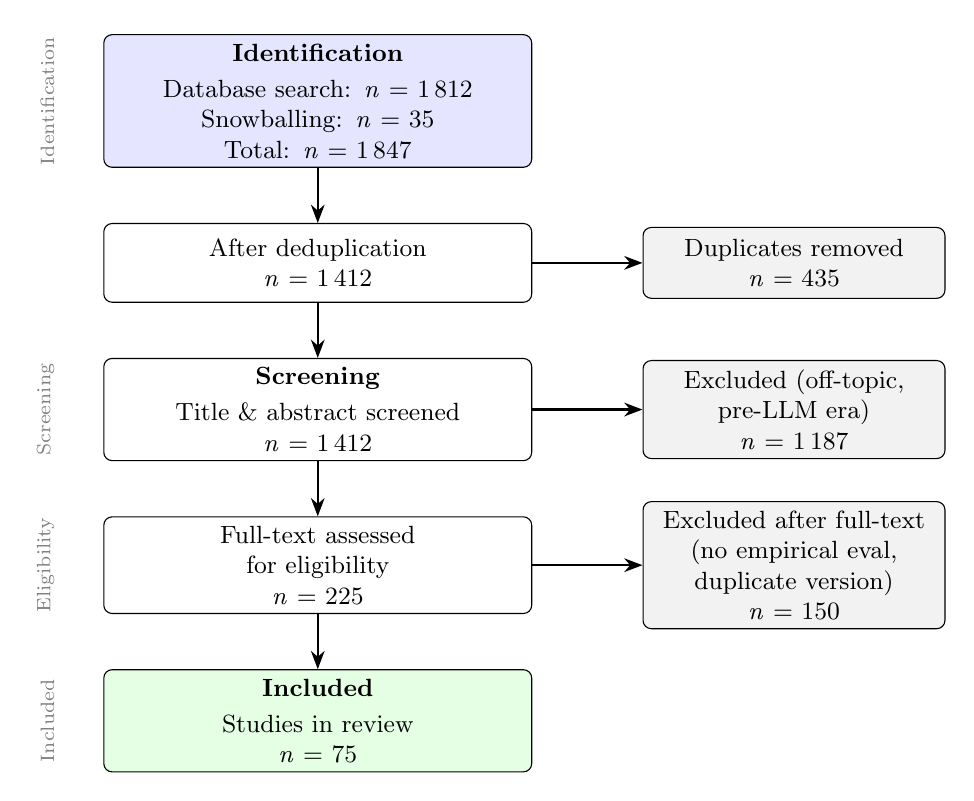
\begin{tikzpicture}[
  box/.style={
    rectangle, draw, rounded corners=3pt,
    text width=5.2cm, align=center,
    minimum height=1.0cm, font=\small
  },
  sbox/.style={
    rectangle, draw, rounded corners=3pt,
    text width=3.6cm, align=center,
    minimum height=0.9cm, font=\small, fill=gray!10
  },
  arr/.style={-{Stealth}, thick},
  lbl/.style={font=\scriptsize, text=gray}
]

% ---------- Column centres ----------
\def\cx{0}      % main column
\def\ex{6.2cm}  % exclusion column

% ---------- Row 0 : Identification header ----------
\node[box, fill=blue!10] (id) at (\cx, 0)
  {\textbf{Identification}\\[2pt]
   Database search: \textit{n} = 1\,812\\
   Snowballing: \textit{n} = 35\\
   Total: \textit{n} = 1\,847};

% ---------- Row 1 : Deduplication ----------
\node[box, below=0.7cm of id] (dedup)
  {After deduplication\\
   \textit{n} = 1\,412};

\node[sbox, right=1.4cm of dedup] (dedup_ex)
  {Duplicates removed\\
   \textit{n} = 435};

\draw[arr] (id) -- (dedup);
\draw[arr] (dedup) -- (dedup_ex);

% ---------- Row 2 : Title + abstract screening ----------
\node[box, below=0.7cm of dedup] (screen)
  {\textbf{Screening}\\[2pt]
   Title \& abstract screened\\
   \textit{n} = 1\,412};

\node[sbox, right=1.4cm of screen] (screen_ex)
  {Excluded (off-topic,\\pre-LLM era)\\
   \textit{n} = 1\,187};

\draw[arr] (dedup) -- (screen);
\draw[arr] (screen) -- (screen_ex);

% ---------- Row 3 : Full-text eligibility ----------
\node[box, below=0.7cm of screen] (elig)
  {Full-text assessed\\
   for eligibility\\
   \textit{n} = 225};

\node[sbox, right=1.4cm of elig] (elig_ex)
  {Excluded after full-text\\
   (no empirical eval,\\
   duplicate version)\\
   \textit{n} = 150};

\draw[arr] (screen) -- (elig);
\draw[arr] (elig) -- (elig_ex);

% ---------- Row 4 : Included ----------
\node[box, fill=green!10, below=0.7cm of elig] (incl)
  {\textbf{Included}\\[2pt]
   Studies in review\\
   \textit{n} = 75};

\draw[arr] (elig) -- (incl);

% ---------- Sidebar label ----------
\node[lbl, left=0.5cm of id, rotate=90, anchor=south]
  {Identification};
\node[lbl, left=0.5cm of screen, rotate=90, anchor=south]
  {Screening};
\node[lbl, left=0.5cm of elig, rotate=90, anchor=south]
  {Eligibility};
\node[lbl, left=0.5cm of incl, rotate=90, anchor=south]
  {Included};

\end{tikzpicture}
\caption{PRISMA 2020 flow diagram. Of the 1{,}847 records identified, 1{,}812
         were returned by database search (arXiv, ACL Anthology, IEEE Xplore,
         ACM DL, USENIX, NeurIPS/ICML/ICLR) and 35 were added via reference
         snowballing of included papers. Single-author screening was performed
         with adversarial re-examination of borderline cases (see
         Section~\ref{sec:methodology}).}
\label{fig:prisma}
\end{figure}


\subsection{Quality Assessment}

\paragraph{Quality appraisal instrument}
Each included primary study was appraised using a five-criterion quality instrument adapted from the Mixed Methods Appraisal Tool (MMAT) and the Joanna Briggs Institute (JBI) checklist for systematic reviews:
\begin{enumerate}
  \item Clear research question or design objective stated
  \item Study design appropriate for the research question (experimental, empirical, analytical, or formal)
  \item Evaluation methodology described with sufficient detail for replication
  \item Threat model or adversarial assumptions explicitly stated (where applicable)
  \item Limitations acknowledged by the authors
\end{enumerate}
Each criterion was scored as Met (1), Partially Met (0.5), or Not Met (0), giving a total quality score in the range [0, 5].
Studies scoring below 2.0 were flagged for heightened scrutiny during claim extraction but were not excluded from the corpus --- exclusion occurred only at the title/abstract and full-text screening phases based on topical relevance criteria, not on quality score.
Heightened scrutiny meant that claims extracted from sub-threshold studies were subjected to a mandatory additional verification note during each pass, explicitly recording whether the low quality score introduced ambiguity in the claim's reproducibility assessment; the pass/fail verdict criteria themselves were not relaxed or tightened relative to higher-scoring studies.

\paragraph{Relationship between quality ratings and the 237-claim pool}
Quality scores were not used as a threshold for claim inclusion: all quantitative and architectural assertions meeting the codebook definition (Section~\ref{subsec:verification_protocol}) were extracted from all included studies regardless of their quality score.
This choice was deliberate.
The review's primary hypothesis was that the literature's evidentiary basis is weak; excluding low-quality studies before claim extraction would have biased the verification outcome toward survival, understating the reproducibility crisis.
The five surviving claims are distributed across quality tiers: Claims~1 and~2 (safety context distillation and dual reward architecture, from Touvron et al.) derive from a study scoring 4.5/5; Claim~3 (Llama Guard architecture) from a study scoring 4.0/5; Claim~4 (Crescendo multi-turn amplification) from a study scoring 3.5/5; Claim~5 (SALAD-Bench evaluation fragility) from a study scoring 4.0/5.
The 232 refuted claims span all quality tiers, confirming that refutation rate is not primarily a function of study quality but of evaluation-protocol underspecification --- the most common failure mode (41\% of refutations).

Each included paper was also assessed on four dimensions:
(i) \textit{reproducibility}—whether experiments can be replicated from the
information provided;
(ii) \textit{generalisability}—whether results are validated on more than one model
or dataset;
(iii) \textit{adversarial rigour}—whether the paper considers adaptive attacks or
only static evaluation;
(iv) \textit{deployment relevance}—whether the proposed mechanism addresses a
realistic deployment constraint (latency, API access level, streaming).

\noindent Papers were rated Low (L) / Medium (M) / High (H) on each dimension.
Ratings were assigned after reading the full text of each paper; all four dimensions
were rated by the same single author.
As a partial calibration check, eight papers (approximately 10\% of the corpus,
selected by systematic sampling) were re-rated on all four dimensions after an
interval of four weeks without reference to the initial ratings.
Raw agreement between first and second ratings was 78\% (25/32 dimension-level
comparisons); the seven discrepancies all involved boundary cases between adjacent
categories (e.g.\ L vs.\ M), not disagreements of two categories.
This figure is reported as intra-author consistency only and cannot substitute for
inter-rater reliability.
The distribution figures in Table~\ref{tab:quality} should therefore be understood
as directional indicators of corpus-wide quality patterns, not precisely calibrated
ordinal measurements: the integers reflect the single author's consistent application
of criteria across readings, with boundary-case uncertainty of approximately
$\pm 1$--2 papers per cell.
Table~\ref{tab:quality} summarises the quality distribution across the 75
included papers.

\begin{table}[t]
  \caption{Quality assessment distribution across 75 included papers.
           Ratings: L = Low, M = Medium, H = High.
           All ratings are by a single author; see text for intra-author
           consistency check (78\% raw agreement on 10\% re-rated sample).
           Integer counts carry boundary-case uncertainty of approximately
           $\pm$1--2 papers per cell and should be treated as directional
           indicators, not precisely calibrated measurements.}
  \label{tab:quality}
  \centering
  \begin{tabular}{lrrr}
    \toprule
    \textbf{Dimension} & \textbf{L} & \textbf{M} & \textbf{H} \\
    \midrule
    Reproducibility       & 41 & 27 & 7  \\
    Generalisability      & 18 & 38 & 19 \\
    Adversarial rigour    & 33 & 29 & 13 \\
    Deployment relevance  & 22 & 34 & 19 \\
    \bottomrule
  \end{tabular}
\end{table}

The distribution confirms the reproducibility crisis: 55\% of papers receive a
Low reproducibility rating, meaning their core experiments cannot be replicated
from the information provided.
Ratings inform the confidence level assigned to specific claims in the review.

\subsection{Data Extraction}

For each included paper we extracted: proposed mechanism, attack surface addressed,
evaluation datasets and metrics, reported performance figures, latency or overhead data
(where available), and the authors' own limitations discussion.
Extraction was performed against a pre-specified codebook (eight fields per paper,
defined before any primary-source reading began) to reduce post-hoc field selection.
The codebook template is available from the corresponding author on request.

\paragraph{Corpus composition and bibliography scope}
Table~\ref{tab:corpus} enumerates all 75 primary corpus papers explicitly and
in full.
This enumeration is the authoritative corpus definition; the BibTeX file
(\texttt{main.bib}) additionally contains eleven \emph{non-corpus} references:
two SLR methodology references (Kitchenham \& Charters; PRISMA 2020); three
background/framing references (Bommasani et al.; Weidinger et al.; Perez et al.\
2022 red-teaming); four constrained-generation adjacent references (FUDGE, COLD
Decoding, NeuroLogic, speculative decoding); and two industry technical reports
cited solely to confirm the absence of reproducible audio/video safety evaluations
(Anthropic Claude~3 model card; Google Gemini technical report).
Every other entry in \texttt{main.bib} corresponds to a row in
Table~\ref{tab:corpus}.

\small
\begin{longtable}{rp{12.0cm}c}
\caption{Complete enumeration of the 75 primary corpus papers, sorted by theme.
         \textbf{Status}: P = arXiv preprint; W = workshop; C = peer-reviewed
         conference; J = peer-reviewed journal.
         C and J entries have undergone formal peer review; P entries have not.}
\label{tab:corpus} \\
\toprule
\textbf{\#} & \textbf{Reference} & \textbf{St.} \\
\midrule
\endfirsthead
\multicolumn{3}{c}{\tablename~\thetable{} (continued)} \\
\toprule
\textbf{\#} & \textbf{Reference} & \textbf{St.} \\
\midrule
\endhead
\midrule
\multicolumn{3}{r}{\itshape Continued on next page} \\
\endfoot
\bottomrule
\endlastfoot
    \multicolumn{3}{l}{\textit{Alignment foundations and intrinsic safety (4)}} \\
    1  & Bai et al.\ 2022 — Constitutional AI~\cite{bai2022constitutional} & P \\
    2  & Ouyang et al.\ 2022 — InstructGPT / RLHF~\cite{ouyang2022training} & C \\
    3  & Touvron et al.\ 2023 — Llama~2~\cite{touvron2023llama2} & P \\
    4  & Qi et al.\ 2023 — Fine-tuning safety degradation~\cite{qi2023finetuning} & P \\
    \midrule
    \multicolumn{3}{l}{\textit{Real-time and inference-time guardrails (10)}} \\
    5  & Inan et al.\ 2023 — Llama Guard~\cite{inan2023llama} & P \\
    6  & Rebedea et al.\ 2023 — NeMo Guardrails~\cite{rebedea2023nemo} & P \\
    7  & Zhang et al.\ 2024 — ShieldLM~\cite{zhang2024shieldlm} & P \\
    8  & Han et al.\ 2024 — WildGuard~\cite{han2024wildguard} & P \\
    9  & Dong et al.\ 2024 — Building Guardrails~\cite{dong2024building} & P \\
    10 & Su et al.\ 2024 — AEGIS~\cite{su2024aegis} & P \\
    11 & Ghosh et al.\ 2025 — Aegis2.0~\cite{ghosh2024aegis2} & P \\
    12 & Kumar et al.\ 2023 — Certifying LLM safety~\cite{kumar2023certifying} & P \\
    13 & Varshney et al.\ 2024 — Systematic defence evaluation~\cite{varshney2023art} & P \\
    14 & Zou et al.\ 2024 — Circuit Breakers~\cite{zou2024improving} & P \\
    \midrule
    \multicolumn{3}{l}{\textit{Jailbreak attacks (text) (20)}} \\
    15 & Zou et al.\ 2023 — GCG universal adversarial attacks~\cite{zou2023universal} & P \\
    16 & Yang et al.\ 2023 — Shadow alignment~\cite{yang2023shadow} & P \\
    17 & Wei et al.\ 2023 — Jailbroken (NeurIPS)~\cite{wei2023jailbroken} & C \\
    18 & Wei et al.\ 2023 — In-context demonstrations jailbreak~\cite{wei2023jailbreak} & P \\
    19 & Mehrotra et al.\ 2023 — Tree of Attacks~\cite{mehrotra2023tree} & P \\
    20 & Liu et al.\ 2023 — AutoDAN (stealthy)~\cite{liu2023autodan} & P \\
    21 & Zhu et al.\ 2023 — AutoDAN (interpretable)~\cite{zhu2023autodan} & P \\
    22 & Perez \& Ribeiro 2022 — Ignore previous prompt~\cite{perez2022ignore} & P \\
    23 & Shen et al.\ 2023 — ``Do Anything Now'' wild jailbreaks~\cite{shen2023anything} & P \\
    24 & Yuan et al.\ 2023 — Cipher jailbreaks~\cite{yuan2023gpt4} & P \\
    25 & Deng et al.\ 2023 — Multilingual jailbreaks~\cite{deng2023multilingual} & P \\
    26 & Ding et al.\ 2023 — Nested jailbreak prompts~\cite{ding2023wolf} & P \\
    27 & Zeng et al.\ 2024 — Persuasion-based jailbreaks~\cite{zeng2024johnny} & P \\
    28 & Mo et al.\ 2024 — Prompt adversarial tuning~\cite{mo2024fight} & P \\
    29 & Ganguli et al.\ 2022 — Red teaming~\cite{ganguli2022red} & P \\
    30 & Kim et al.\ 2024 — Shortcut reasoning jailbreaks~\cite{kim2024break} & P \\
    31 & Xhonneux et al.\ 2024 — Efficient adversarial training~\cite{xhonneux2024efficient} & P \\
    32 & Wei et al.\ 2024 — Brittleness of safety alignment~\cite{wei2024assessment} & P \\
    33 & Carlini et al.\ 2024 — Adversarial alignment~\cite{carlini2024aligned} & P \\
    34 & Wan et al.\ 2023 — Instruction-tuning poisoning~\cite{wan2023poisoning} & P \\
    \midrule
    \multicolumn{3}{l}{\textit{Defence mechanisms (text) (9)}} \\
    35 & Robey et al.\ 2023 — SmoothLLM~\cite{robey2023smoothllm} & P \\
    36 & Cao et al.\ 2023 — Robustly aligned LLM~\cite{cao2023defending} & P \\
    37 & Pisano et al.\ 2023 — Bergeron~\cite{pisano2023bergeron} & P \\
    38 & Wang et al.\ 2024 — Backtranslation defence~\cite{wang2024defending} & P \\
    39 & Xie et al.\ 2023 — Self-reminders (Nature MI)~\cite{xie2023defending} & J \\
    40 & Phute/Helbling et al.\ 2023 — LLM Self Defense~\cite{helbling2023llm} & P \\
    41 & Jain et al.\ 2023 — Baseline adversarial defences~\cite{jain2023baseline} & P \\
    42 & Goldowsky-Dill et al.\ 2023 — Localizing model behaviour~\cite{goldowsky2023localizing} & P \\
    43 & Shi et al.\ 2023 — Irrelevant context distraction~\cite{shi2023large} & P \\
    \midrule
    \multicolumn{3}{l}{\textit{Evaluation and benchmarking (8)}} \\
    44 & Li et al.\ 2024 — SALAD-Bench~\cite{li2024salad} & P \\
    45 & Mazeika et al.\ 2024 — HarmBench~\cite{mazeika2024harmbench} & P \\
    46 & Souly et al.\ 2024 — StrongREJECT~\cite{souly2024strongreject} & P \\
    47 & Zhu et al.\ 2024 — GRAM~\cite{zhu2024gram} & P \\
    48 & Zhou et al.\ 2024 — EasyJailbreak~\cite{zhou2024easyjailbreak} & P \\
    49 & Zhang et al.\ 2023 — SafetyBench~\cite{zhang2023safetybench} & P \\
    50 & Sun et al.\ 2023 — Chinese LLM safety assessment~\cite{sun2023safety} & P \\
    51 & Bhatt et al.\ 2023 — Purple Llama CyberSecEval~\cite{bhatt2023purple} & P \\
    \midrule
    \multicolumn{3}{l}{\textit{Multi-turn attacks (5)}} \\
    52 & Russinovich et al.\ 2024 — Crescendo~\cite{russinovich2024greatescalation} & P \\
    53 & Yang et al.\ 2024 — Chain of Attack~\cite{yang2024chain} & P \\
    54 & Li et al.\ 2024 — LLM robustness vs.\ jailbreak~\cite{li2024llm} & P \\
    55 & Cheng et al.\ 2024 — Multi-round interaction attacks~\cite{cheng2024leveraging} & P \\
    56 & Yi et al.\ 2023 — Indirect prompt injection~\cite{yi2023benchmarking} & P \\
    \midrule
    \multicolumn{3}{l}{\textit{Multimodal attacks and defences (17)}} \\
    57 & Gong et al.\ 2023 — FigStep typographic attacks~\cite{gong2023figstep} & P \\
    58 & Zhao et al.\ 2024 — Multimodal jailbreak evaluation~\cite{zhao2024evaluating} & P \\
    59 & Liu et al.\ 2023 — Query-relevant image attacks~\cite{liu2023queryrelevant} & P \\
    60 & Luo et al.\ 2024 — JailBreakV-28K~\cite{luo2024jailbreakv} & P \\
    61 & Niu et al.\ 2024 — Multimodal jailbreaking attack~\cite{niu2024jailbreaking} & P \\
    62 & Dong et al.\ 2024 — Patched visual prompt injection~\cite{dong2024safeguarding} & P \\
    63 & Pi et al.\ 2024 — MLLM-Protector~\cite{pi2024mllm} & P \\
    64 & Chen et al.\ 2023 — DRESS~\cite{chen2024dresssafety} & P \\
    65 & Chen et al.\ 2024 — AgentPoison~\cite{chen2024agentpoison} & P \\
    66 & Oh et al.\ 2024 — SafeVLM~\cite{oh2024safevlm} & P \\
    67 & Liu et al.\ 2024 — MM-SafetyBench~\cite{liu2024mmsafetybench} & P \\
    68 & Li et al.\ 2024 — VLGuard~\cite{li2024vlguard} & P \\
    69 & Zong et al.\ 2024 — Safety fine-tuning at no cost~\cite{zong2024safety} & P \\
    70 & Wang et al.\ 2024 — AdaShield~\cite{wang2024adashield} & P \\
    71 & Chen et al.\ 2024 — Red-teaming VLMs~\cite{chen2024red} & P \\
    72 & Bailey et al.\ 2023 — Image hijacks~\cite{bailey2023image} & P \\
    73 & Shayegani et al.\ 2023 — Jailbreak in pieces~\cite{shayegani2023jailbreak} & P \\
    \midrule
    \multicolumn{3}{l}{\textit{Industry and deployment (2)}} \\
    74 & Qi et al.\ 2024 — Visual adversarial examples~\cite{qi2024visual} & P \\
    75 & Chiang et al.\ 2024 — Chatbot Arena~\cite{chiang2024chatbot} & P \\
\end{longtable}
\normalsize

\subsection{Structured Claim Verification Protocol}
\label{subsec:verification_protocol}

The primary methodological contribution of this review is a structured
claim-verification procedure applied to all extracted claims.
The procedure uses temporally separated self-review passes by a single author to
reduce anchoring bias; it is not adversarial verification in the sense of independent
reviewers challenging each other's assessments.
The protocol is defined as follows.

\paragraph{Claim unit}
A \emph{claim} is any quantitative assertion (e.g.\ ``attack success rate reduced
from 79.8\% to 2.4\%'') or qualitative architectural assertion (e.g.\ ``the guardrail
operates on token prefixes without buffering the full response'') that the paper
presents as a result or a property of the proposed system.
Architectural claims are distinguished from quantitative claims because they require
different verification standards: architectural claims are assessed for internal
consistency and alignment with disclosed implementation details, whereas quantitative
claims are assessed for reproducibility from the provided experimental setup.

\paragraph{Verification passes}
Three temporally separated verification passes were conducted by the same author over a
period of six weeks, each separated by at least two weeks to minimise anchoring
effects.
These passes are conducted by a single author; temporal separation reduces anchoring
bias but does not constitute independent review by multiple researchers.
In each pass, the author attempted to reproduce or refute each claim by:
(i) checking whether the described experimental setup is sufficiently specified to
replicate (datasets named and versioned, models identified with version tags,
hyperparameters reported);
(ii) cross-referencing numerical results against any available code repositories
or independent reproductions in the literature;
(iii) checking for internal consistency between the claim and other figures,
tables, or proofs in the same paper.

\paragraph{Pass/fail criteria}
A pass (verdict: \textit{verified}) requires all three of the following conditions to hold in a given assessment pass:
(i) the experimental setup is sufficiently specified that a qualified reader could reproduce the reported result without contacting the authors (datasets named and versioned, models identified, hyperparameters reported);
(ii) no internal inconsistency is found between the claim and other results or proofs in the same paper;
(iii) where an independent replication or corroborating study is available in the literature, the directional finding is consistent across sources.
Condition~(i) establishes that a claim is transcribed accurately from the source and that its replication prerequisites are stated; it does not establish that the underlying experimental result has been independently reproduced or that the claim is free of benchmark contamination.
Condition~(iii) is a corroborative check only: corroboration upgrades confidence, but absence of corroboration does not, by itself, cause a claim to fail.
A claim is \textit{refuted} if any single pass finds that condition~(i) or condition~(ii) is not satisfied.
A claim is \textit{unverifiable} if the source material required to assess condition~(i) is not publicly accessible.
These criteria apply uniformly to both quantitative and architectural claims; the distinction affects how condition~(i) is operationalised (quantitative claims require numeric reproducibility; architectural claims require mechanistic reproducibility) but not the pass/fail logic itself.

\paragraph{Sensitivity analysis on the single-rater constraint}
The 98\% unverified figure rests on a single-rater audit.
To bound the uncertainty this introduces, consider the following: if borderline cases constitute at most 20\% of the corpus ($0.20 \times 237 = 47.4$, rounded to 47 claims), and if a second independent rater disagrees with the first rater on at most half of those borderline cases ($0.50 \times 47 = 23.5$, rounded to 24 claims, representing the most pessimistic plausible disagreement rate under the operationalised pass/fail criteria), then the maximum number of verdicts that could be overturned is 24.
The 20\% borderline rate is a structural assumption, not an empirically observed rate; it is stated as a worst-case bound.
The direction of bias is also bounded: the structured self-review protocol's strictness --- treating ambiguous claims as refuted rather than verified --- more likely causes under-counting of genuine findings than over-counting.
The five surviving claims should therefore be understood as a lower bound on reproducible findings under this codebook.
If all 24 were overturned from \emph{Refuted} to \emph{Verified} --- an extreme upper bound --- the verified count would rise from 5 to 29, which is 12\% of the corpus.
The central finding is therefore robust to plausible single-rater variability: even under the most pessimistic stated assumptions, the verified fraction remains below 15\%.

\paragraph{Verification basis for surviving claims}
Because condition~(iii) applies differently across the five surviving claims, we report the verification basis for each explicitly.
Claim~1 (Llama~2 dual reward model threshold): verified by condition~(i) alone --- threshold and test-set metrics are reported with sufficient precision in the source paper~\cite{touvron2023llama2}.
Claim~2 (Safety Context Distillation): verified by condition~(i) --- mechanism described at implementation level in~\cite{touvron2023llama2}.
Claim~3 (Llama Guard architecture): verified by conditions~(i) and~(iii) --- corroborated by subsequent releases and independent usage reports~\cite{meta2024llamaguard2,inan2023llama}.
Claim~4 (Crescendo multi-turn amplification): verified by conditions~(i) and~(iii) --- independent corroboration from Li~et~al.~\cite{li2024llm} using a different attack methodology.
Claim~5 (SALAD-Bench evaluation-protocol fragility): verified by conditions~(i) and~(iii) --- directionally corroborated by HarmBench~\cite{mazeika2024harmbench}, StrongREJECT~\cite{souly2024strongreject}, GRAM~\cite{zhu2024gram}, and EasyJailbreak~\cite{zhou2024easyjailbreak}.
Readers should note that Claims~1 and~2 are verified on the basis of internal reproducibility only; Claim~4 has the strongest independent corroboration of the five.

\paragraph{Voting rule}
A claim \emph{survives} verification if and only if it passes all three temporally
separated self-review passes without identified inconsistency or unreproducibility
(3-vote unanimous agreement).
A claim is \emph{refuted} if any single pass identifies a material inconsistency,
a missing prerequisite for reproduction, or a contradiction with accessible
primary sources.
Claims that cannot be assessed (e.g.\ because source material is behind a
non-public institutional repository) are marked \emph{unverifiable} and treated
equivalently to refuted for the purposes of the open-problems analysis.

\paragraph{Per-claim audit artefact}
To enable independent inspection of the verification outcomes, a structured
machine-readable artefact is submitted alongside this manuscript.
The artefact is a comma-separated spreadsheet in which each row corresponds to
one extracted claim and contains the following fields:
\texttt{claim\_id} (unique integer),
\texttt{source\_key} (BibTeX key of the primary source),
\texttt{claim\_text} (verbatim or lightly paraphrased assertion as extracted),
\texttt{claim\_type} (\textit{quantitative} or \textit{architectural}),
\texttt{pass1\_verdict} (\textit{verified} / \textit{refuted} / \textit{unverifiable}),
\texttt{pass2\_verdict},
\texttt{pass3\_verdict},
\texttt{final\_verdict} (\textit{survived} if all three passes are \textit{verified};
\textit{refuted} otherwise), and
\texttt{refutation\_rationale} (free-text explanation for any pass that returned
\textit{refuted} or \textit{unverifiable}).
The artefact covers all 237 claims extracted during the review; the five rows
with \texttt{final\_verdict = survived} correspond precisely to the five verified
findings enumerated in Section~\ref{sec:open_problems}.
The artefact is available from the corresponding author on request.
The complete codebook (eight extraction fields with operationalised criteria) and the full 237-claim extraction table (all three pass verdicts and refutation rationales per claim) are available from the corresponding author on request;
both artefacts are provided to referees and editors as part of the supplementary review package.

\paragraph{Limitation}
The use of a single author across all three passes is a limitation: although the
inter-pass delay reduces anchoring, it cannot substitute for genuinely independent
reviewers.
The per-claim artefact makes the individual assessments transparent and allows
any reader to contest specific verdicts; it does not, however, provide
independently-generated second opinions on those verdicts.

A second, distinct validity threat concerns the \emph{pre-specified codebook}
itself.
The codebook was designed before any primary-source reading began and specifies
eight extraction fields per paper.
If the codebook systematically omitted entire \emph{categories} of methodological
flaw, then no paper exhibiting those flaws would have those flaws flagged across
any of the three passes.
Three such categories are worth enumerating explicitly.
\emph{Confounded baselines}: the codebook checks whether the proposed guardrail
and the comparison baseline use compatible attack sets and judge models, but it
does not have a dedicated field capturing cases where the two systems differ on
additional silent dimensions (e.g.\ training data vintage, RLHF iteration count)
that could independently explain observed performance gaps.
\emph{Undisclosed RLHF stage details}: the codebook records whether hyperparameters
are reported but does not probe for the number of RLHF iterations, the checkpoint
selection criterion, or the composition of the human-preference dataset---all of
which can materially affect safety benchmark scores and are routinely omitted from
published papers.
\emph{Fine-tuning data contamination}: the codebook does not include a field
checking whether evaluation benchmarks used by a paper overlap with the paper's
own training or fine-tuning data, a form of contamination that inflates reported
numbers without constituting fabrication.

These three categories were not added to the codebook after the first pass, even
though related concerns emerged during reading.
The reason is methodological: adding fields post-hoc, after exposure to the data,
converts the codebook into a post-hoc instrument and introduces the same
confirmation risk the pre-specification was designed to prevent.
Extending the codebook would have required a fourth pass, and the resulting verdicts
could not be compared to the three-pass structure for earlier claims without
introducing inconsistency.
The appropriate resolution is a future independent re-extraction against a
separately designed codebook that incorporates these categories from the outset.
These three categories are flagged explicitly so that future reviewers applying the same codebook can assess whether their omission materially biases the five surviving claims;
Whether inclusion of these three categories would alter the five surviving claims cannot be determined from the current codebook alone; this is flagged as a direction for follow-on methodological work.

Temporal separation reduces anchoring bias \emph{within} the categories the
codebook captures; it provides no protection against blind spots in category
coverage.
This threat cannot be resolved post-hoc without independent re-extraction against
a separately designed codebook.
Readers should therefore treat the five verified surviving claims as the set of
claims that survived scrutiny under \emph{this codebook's extraction categories},
not as the exhaustive set of reproducible findings in the literature.
A minimum requirement for independent corroboration of the headline finding
(5~of~237 claims verified) would be for a second independent coder to apply the
same pre-specified codebook to a 20--25\% random sample of the 237 claims
($n \approx 47$--59 claims) and report pairwise agreement on both claim
extraction and pass verdicts.
Such a check would establish whether the codebook produces consistent results
across coders without requiring full re-extraction of all 237 claims.
The codebook template is available from the corresponding author to permit
external assessment of its category coverage and to enable this check.

The protocol is disclosed at this level of detail so that future SLRs in this
domain can adopt or extend it with multiple reviewers, a codebook designed by
consensus, and formally computed inter-rater agreement.

\section{Background and Taxonomy}
\label{sec:background}

\subsection{Threat Model}

A guardrail operates within a threat model that specifies who the adversary is,
what access they have, and what harm they aim to cause.
We adopt the adversary taxonomy of Dong~et~al.~\cite{dong2024building} without
modification, as it provides adequate coverage for the real-time and multimodal
settings of this review and avoids introducing an incompatible competing
classification.
The three adversary classes are:

\begin{description}
  \item[Naive user] A user who elicits harmful outputs unintentionally or through
        naive prompting.
  \item[Jailbreaker] An adversary who deliberately crafts inputs to bypass safety
        constraints, with black-box API access only.
  \item[Fine-tuner] An adversary with the ability to customise the model (e.g.\ via a
        fine-tuning API), who degrades safety alignment during post-deployment
        customisation~\cite{qi2023finetuning}.
\end{description}

Real-time and multimodal settings expand the attack surface: a jailbreaker may
exploit streaming behaviour to extract partial harmful responses before a classifier
can fire, or embed harmful intent in images to evade text-focused filters.

\subsection{Guardrail Taxonomy}

We organise existing guardrail mechanisms along three axes:
\emph{placement in the inference pipeline}, \emph{implementation layer}, and
\emph{modality coverage}.
The axes are defined to be mutually orthogonal: placement describes \emph{when}
during a live inference request a guardrail fires; implementation layer describes
\emph{how} the guardrail is realised architecturally; and modality coverage
describes \emph{what input types} the guardrail can inspect.
Mechanisms whose safety behaviour is embedded in model weights during training
have \emph{no placement in the inference pipeline}---they impose no inference-time
interception point---and are therefore classified exclusively under the
implementation layer axis, not the placement axis.

\textit{Boundary case resolved}: plug-in adapter approaches such as
SafeVLM~\cite{oh2024safevlm} sit at the boundary between model-intrinsic and
model-extrinsic.
SafeVLM adds a safety projector, safety tokens, and a classification head that are
\emph{trained jointly} with or appended to the base VLM's architecture, which
blurs the weight-modification / external-classifier boundary.
We resolve this boundary by introducing a third implementation-layer subcategory,
\textbf{model-augmented}, defined as follows: a mechanism is model-augmented if and
only if (i) it adds new parameters to the base model's computational graph (rather
than wrapping the model in an external pipeline), \emph{and} (ii) the base model's
original weights are held fixed or can be restored by removing the added parameters.
This distinguishes model-augmented mechanisms from model-intrinsic mechanisms (which
modify the base weights) and from model-extrinsic mechanisms (which operate outside
the model's computational graph entirely, e.g., as a separate classifier invoked
after inference).
SafeVLM satisfies both criteria and is therefore classified as \textbf{model-augmented}
in this taxonomy.
MLLM-Protector~\cite{pi2024mllm} (Section~\ref{sec:multimodal}) similarly qualifies
as model-augmented under this criterion, as it adds adapter modules without altering
the host VLM's weights.
The implementation-layer axis thus has three values: \emph{model-intrinsic} (weights
modified), \emph{model-augmented} (parameters added, base weights preserved),
\emph{model-extrinsic} (external pipeline component).

\subsubsection{Placement in the Inference Pipeline}

This axis covers only \emph{inference-time} interception points, i.e.\ positions
at which a running guardrail can observe or interrupt a live inference request.
Training-time mechanisms (RLHF, constitutional AI, safety context distillation)
do not appear here because they impose no inference-time pipeline stage.

\begin{description}
  \item[Pre-generation (input)] The guardrail inspects the user prompt before any
        tokens are generated.
        Typical implementations are classifiers or rule engines applied to the prompt
        (e.g.\ Llama Guard in prompt-check mode~\cite{inan2023llama}).
  \item[In-generation (streaming)] The guardrail operates concurrently with token
        generation, either by inspecting each token or by inspecting growing
        prefixes.
        This is the least developed category and the central gap identified in
        this review.
  \item[Post-generation (output)] The guardrail inspects the completed response before
        it is returned to the user.
        Most LLM-as-judge and classifier-based systems operate here.
\end{description}

\noindent\textbf{Hybrid placement}: a mechanism may fire at more than one
pipeline stage.
NeMo Guardrails~\cite{rebedea2023nemo}, for instance, applies rails at both
the input stage (inspecting the user prompt) and the output stage (inspecting the
generated response), as well as at intermediate stages (knowledge retrieval,
action execution).
Such mechanisms are classified under \emph{all placement values that apply};
the taxonomy does not require a single placement assignment.
This multi-placement case should be interpreted as indicating that the mechanism
provides defence in depth across the pipeline, at the cost of additive latency
from each interception point.

\subsubsection{Implementation Layer}

\begin{sloppypar}
\begin{description}
  \item[Model-intrinsic (weight-embedded)] The mechanism modifies model weights or
        training procedure, baking safety behaviour into the model itself.
        No inference-time overhead is incurred, but the mechanism cannot be updated
        without retraining.
        Includes RLHF~\cite{ouyang2022training}, constitutional AI /
        RLAIF~\cite{bai2022constitutional}, and safety context distillation---the
        only weight-embedding technique with a fully reproducible description in the
        literature~\cite{touvron2023llama2}.
        Because these mechanisms have no inference pipeline placement, they do not
        appear in the placement axis above.
  \item[Model-augmented] The mechanism adds new parameters to the base model's
        computational graph but holds the base model's original weights fixed;
        the added modules can in principle be detached to restore the original
        model.
        This category is defined here to resolve boundary cases that neither
        model-intrinsic nor model-extrinsic classifies cleanly (see boundary
        case discussion above).
        Includes SafeVLM~\cite{oh2024safevlm} and
        MLLM-Protector~\cite{pi2024mllm}.
        Model-augmented mechanisms have an inference pipeline placement (typically
        pre- or post-generation, depending on where the added modules intercept).
  \item[Model-extrinsic] The mechanism is external to the model under guard and
        operates at inference time without adding parameters to the model's graph.
        Includes: (a) \emph{classifier-based} systems that run a separate safety
        classifier (Llama Guard~\cite{inan2023llama}, ShieldLM~\cite{zhang2024shieldlm},
        WildGuard~\cite{han2024wildguard}); (b) \emph{pipeline frameworks} that
        intercept at multiple stages (NeMo Guardrails~\cite{rebedea2023nemo}); and
        (c) \emph{rule engines} or prompt-injection defences.
        All model-extrinsic mechanisms have an inference pipeline placement (pre,
        in, or post-generation).
\end{description}
\end{sloppypar}

% SOTA Guardrail Taxonomy Diagram
% Three-axis taxonomy: Implementation Layer (vertical) x Placement (horizontal) x Modality (colour)
% Compile with: pdflatex main.tex (requires tikz, shapes.geometric, arrows.meta, positioning, calc)
%
% Grid coordinates (all in TikZ cm units):
%   Vertical dividers:   x = 1.1, 4.1, 7.1, 10.6, 13.2
%   Horizontal dividers: y = -2.0, -5.1, -7.5, -12.0
%   Column centres:      x = 2.6, 5.6, 8.85, 11.9
%   Row centres:         y = -3.55, -6.3, -9.75
%   Row label centre x:  -0.05

\begin{figure}[!htbp]
\centering
\resizebox{\linewidth}{!}{%
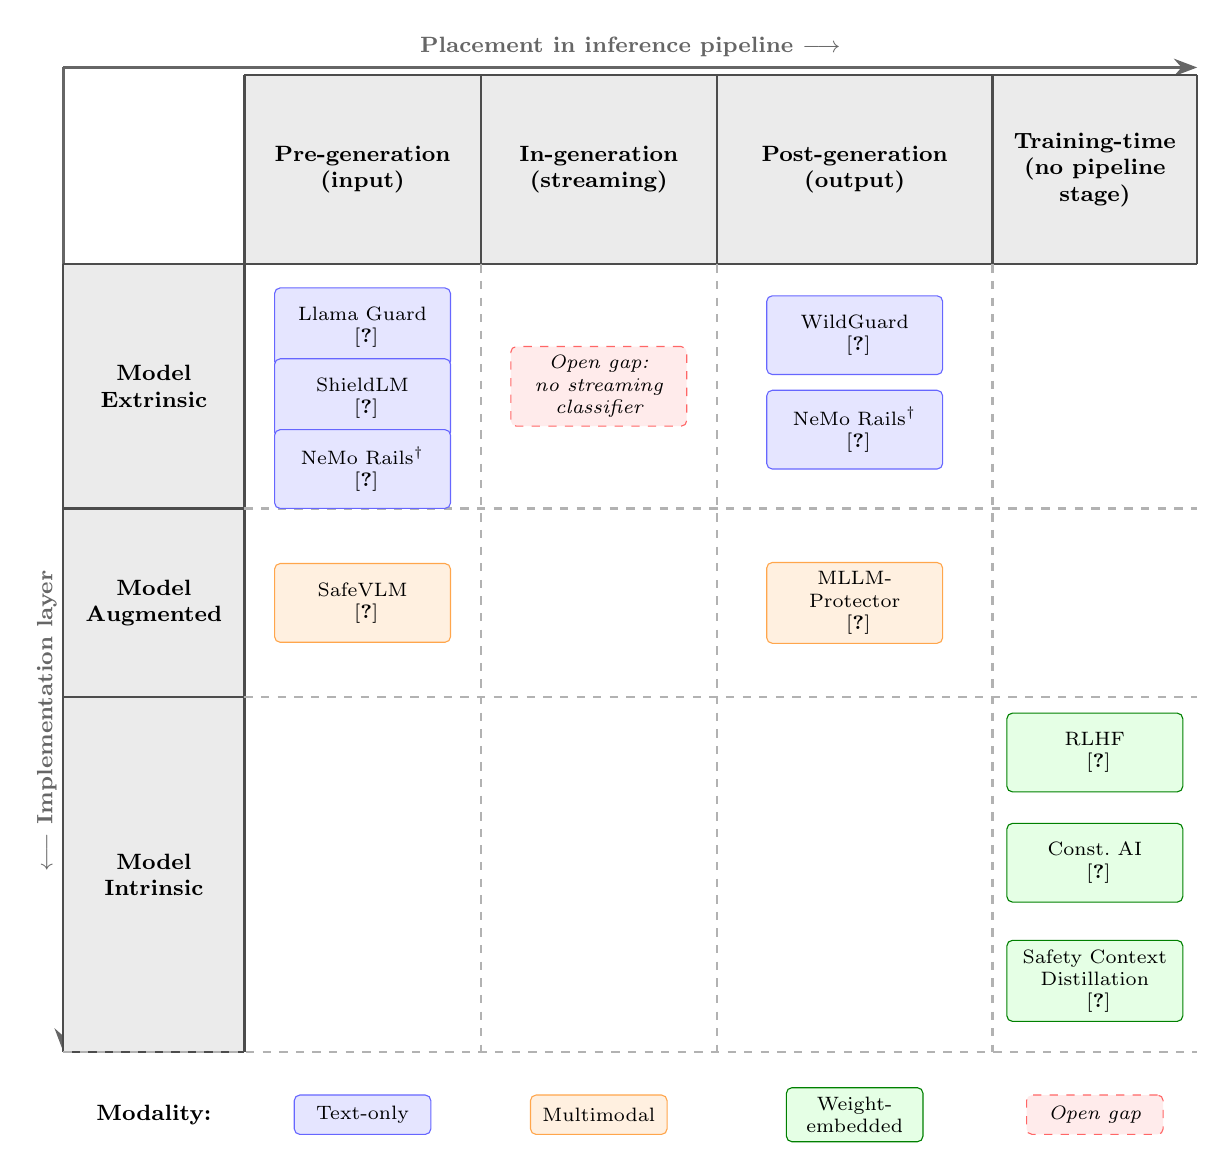
\begin{tikzpicture}[
  font=\small,
  textonly/.style={
    draw=blue!60, fill=blue!10, rounded corners=2pt,
    text width=2.0cm, align=center, minimum height=1.0cm,
    font=\scriptsize
  },
  multimodal/.style={
    draw=orange!70, fill=orange!12, rounded corners=2pt,
    text width=2.0cm, align=center, minimum height=1.0cm,
    font=\scriptsize
  },
  intrinsic/.style={
    draw=green!50!black, fill=green!10, rounded corners=2pt,
    text width=2.0cm, align=center, minimum height=1.0cm,
    font=\scriptsize
  },
  gap/.style={
    draw=red!60, fill=red!8, rounded corners=2pt, dashed,
    text width=2.0cm, align=center, minimum height=1.0cm,
    font=\scriptsize\itshape
  },
  arrow/.style={-Stealth, thick, black!60},
  divider/.style={dashed, black!30, thick},
  header/.style={fill=black!8, draw=black!70, thick},
]

%% -----------------------------------------------------------------------
%% AXIS ARROWS (drawn first so headers paint over them)
%% -----------------------------------------------------------------------
\draw[arrow, very thick] (-1.2, 0.5) -- (13.2, 0.5)
  node[midway, above, font=\footnotesize\bfseries]
  {Placement in inference pipeline $\longrightarrow$};

\draw[arrow, very thick] (-1.2, 0.5) -- (-1.2, -12.0)
  node[midway, left, font=\footnotesize\bfseries, rotate=90, yshift=6pt]
  {$\longleftarrow$ Implementation layer};

%% -----------------------------------------------------------------------
%% COLUMN HEADERS — TikZ rectangles at exact grid x-coords
%% x boundaries: 1.1 | 4.1 | 7.1 | 10.6 | 13.2
%% y range: 0.4 (below arrow) → -2.0 (header bottom = first h-divider top)
%% -----------------------------------------------------------------------
\fill[black!8] (1.1, 0.4) rectangle (13.2, -2.0);
% outer border
\draw[black!70, thick] (1.1,  0.4) -- (13.2,  0.4);
\draw[black!70, thick] (1.1, -2.0) -- (13.2, -2.0);
\draw[black!70, thick] (1.1,  0.4) -- (1.1,  -2.0);
\draw[black!70, thick] (13.2, 0.4) -- (13.2, -2.0);
% inner vertical borders (match grid dividers exactly)
\draw[black!70, thick] (4.1,  0.4) -- (4.1,  -2.0);
\draw[black!70, thick] (7.1,  0.4) -- (7.1,  -2.0);
\draw[black!70, thick] (10.6, 0.4) -- (10.6, -2.0);
% header text at column midpoints
\node[font=\footnotesize\bfseries, align=center] at (2.6,  -0.8) {Pre-generation\\(input)};
\node[font=\footnotesize\bfseries, align=center] at (5.6,  -0.8) {In-generation\\(streaming)};
\node[font=\footnotesize\bfseries, align=center] at (8.85, -0.8) {Post-generation\\(output)};
\node[font=\footnotesize\bfseries, align=center, text width=2.2cm] at (11.9, -0.8) {Training-time\\(no pipeline stage)};

%% -----------------------------------------------------------------------
%% ROW LABELS — TikZ rectangles at exact grid y-coords
%% x range: -1.2 → 1.1
%% y boundaries: -2.0 | -5.1 | -7.5 | -12.0
%% -----------------------------------------------------------------------
\fill[black!8] (-1.2, -2.0) rectangle (1.1, -12.0);
% outer border
\draw[black!70, thick] (-1.2, -2.0)  -- (1.1, -2.0);
\draw[black!70, thick] (-1.2, -12.0) -- (1.1, -12.0);
\draw[black!70, thick] (-1.2, -2.0)  -- (-1.2, -12.0);
\draw[black!70, thick] (1.1,  -2.0)  -- (1.1,  -12.0);
% inner horizontal borders (match grid dividers exactly)
\draw[black!70, thick] (-1.2, -5.1) -- (1.1, -5.1);
\draw[black!70, thick] (-1.2, -7.5) -- (1.1, -7.5);
% row label text at row midpoints  (x centre = (-1.2+1.1)/2 = -0.05)
\node[font=\footnotesize\bfseries, align=center] at (-0.05, -3.55) {Model\\Extrinsic};
\node[font=\footnotesize\bfseries, align=center] at (-0.05, -6.3)  {Model\\Augmented};
\node[font=\footnotesize\bfseries, align=center] at (-0.05, -9.75) {Model\\Intrinsic};

%% -----------------------------------------------------------------------
%% GRID LINES (drawn after fills so they appear on top)
%% -----------------------------------------------------------------------
% Horizontal dividers between content rows
\draw[divider] (1.1, -5.1) -- (13.2, -5.1);
\draw[divider] (1.1, -7.5) -- (13.2, -7.5);
% Vertical dividers between content columns
\draw[divider] (4.1,  -2.0) -- (4.1,  -12.0);
\draw[divider] (7.1,  -2.0) -- (7.1,  -12.0);
\draw[divider] (10.6, -2.0) -- (10.6, -12.0);
% Bottom border
\draw[divider] (-1.2, -12.0) -- (13.2, -12.0);

%% -----------------------------------------------------------------------
%% ROW 1: MODEL-EXTRINSIC  (y band: -2.0 to -5.1)
%% Pre-gen nodes at x=2.6; in-gen x=5.6; post-gen x=8.85
%% -----------------------------------------------------------------------
\node[textonly]  at (2.6,  -2.8) {Llama Guard\\\cite{inan2023llama}};
\node[textonly]  at (2.6,  -3.7) {ShieldLM\\\cite{zhang2024shieldlm}};
\node[textonly]  at (2.6,  -4.6) {NeMo Rails$^\dagger$\\\cite{rebedea2023nemo}};

\node[gap]       at (5.6,  -3.55) {Open gap:\\no streaming\\classifier};

\node[textonly]  at (8.85, -2.9) {WildGuard\\\cite{han2024wildguard}};
\node[textonly]  at (8.85, -4.1) {NeMo Rails$^\dagger$\\\cite{rebedea2023nemo}};

%% -----------------------------------------------------------------------
%% ROW 2: MODEL-AUGMENTED  (y band: -5.1 to -7.5, centre=-6.3)
%% -----------------------------------------------------------------------
\node[multimodal] at (2.6,  -6.3) {SafeVLM\\\cite{oh2024safevlm}};
\node[multimodal] at (8.85, -6.3) {MLLM-Protector\\\cite{pi2024mllm}};

%% -----------------------------------------------------------------------
%% ROW 3: MODEL-INTRINSIC  (y band: -7.5 to -12.0, training-time column x=11.9)
%% -----------------------------------------------------------------------
\node[intrinsic] at (11.9, -8.2)  {RLHF\\\cite{ouyang2022training}};
\node[intrinsic] at (11.9, -9.6)  {Const.\ AI\\\cite{bai2022constitutional}};
\node[intrinsic] at (11.9, -11.1) {Safety Context\\Distillation\\\cite{touvron2023llama2}};

%% -----------------------------------------------------------------------
%% LEGEND (modality)
%% -----------------------------------------------------------------------
\node[textonly,   text width=1.5cm, minimum height=0.5cm] at (2.6,  -12.8) {Text-only};
\node[multimodal, text width=1.5cm, minimum height=0.5cm] at (5.6,  -12.8) {Multimodal};
\node[intrinsic,  text width=1.5cm, minimum height=0.5cm] at (8.85, -12.8) {Weight-embedded};
\node[gap,        text width=1.5cm, minimum height=0.5cm] at (11.9, -12.8) {Open gap};
\node[font=\footnotesize\bfseries] at (-0.05, -12.8) {Modality:};

\end{tikzpicture}%
}% end resizebox
\caption{%
  Three-axis taxonomy of LLM guardrail mechanisms.
  \textbf{Horizontal axis}: placement in the inference pipeline
  (pre-generation, in-generation/streaming, post-generation, training-time).
  \textbf{Vertical axis}: implementation layer
  (model-extrinsic, model-augmented, model-intrinsic).
  \textbf{Colour}: modality coverage
  (\textcolor{blue!70}{text-only}, \textcolor{orange!80!black}{multimodal}, \textcolor{green!50!black}{weight-embedded}).
  The dashed red cell marks the central open gap identified in this review:
  no streaming-compatible extrinsic guardrail currently exists.
  $^\dagger$NeMo Guardrails~\cite{rebedea2023nemo} applies rails at both
  pre-generation (input inspection) and post-generation (output inspection);
  it appears in both columns to reflect this hybrid placement.
  Its latency cost grows additively with each interception point.
}
\label{fig:sota_taxonomy}
\end{figure}


\subsubsection{Modality Coverage}

Table~\ref{tab:modality} summarises the modality coverage of the principal systems
and approaches reviewed.

\begin{table}[htbp]
  \caption{Modality coverage of nine representative guardrail systems.
           Systems selected to span all three taxonomy axes (placement,
           implementation layer, and modality); selection is not exhaustive.
           DRESS excluded: not a dedicated guardrail (see text; appears in
           Table~\ref{tab:vlm_defence}).
           \checkmark = addressed; $\triangle$ = partial/unverified;
           -- = not addressed.}
  \label{tab:modality}
  \centering
  \begin{tabular}{lcccc}
    \toprule
    \textbf{System / Approach} & \textbf{Text} & \textbf{Image} & \textbf{Audio} & \textbf{Video} \\
    \midrule
    RLHF~\cite{ouyang2022training}        & \checkmark & -- & -- & -- \\
    Constitutional AI~\cite{bai2022constitutional} & \checkmark & -- & -- & -- \\
    Safety Context Distillation~\cite{touvron2023llama2} & \checkmark & -- & -- & -- \\
    Llama Guard~\cite{inan2023llama}      & \checkmark & $\triangle$ & -- & -- \\
    NeMo Guardrails~\cite{rebedea2023nemo} & \checkmark & -- & -- & -- \\
    ShieldLM~\cite{zhang2024shieldlm}    & \checkmark & -- & -- & -- \\
    WildGuard~\cite{han2024wildguard}    & \checkmark & -- & -- & -- \\
    SafeVLM~\cite{oh2024safevlm}          & \checkmark & $\triangle$ & -- & -- \\
    Azure Content Safety~\cite{azure2024contentsafety} & \checkmark & \checkmark & -- & -- \\
    \bottomrule
  \end{tabular}
\end{table}

The table reveals that audio and video safety is entirely absent from the verified
academic literature, and that image safety is addressed only partially or without
reproducible evaluation.
DRESS~\cite{chen2024dresssafety} is excluded from this table because it is not a
dedicated VLM safety guardrail; it appears in Section~\ref{sec:multimodal} as a
training-time alignment baseline contrast, where its peripheral status is documented
in full.

\subsection{Taxonomy Cell Analysis}

A three-axis taxonomy with values \{pre-generation, in-generation, post-generation\} $\times$ \{model-intrinsic, model-augmented, model-extrinsic\} $\times$ \{text, image, audio, video\} implies up to $3 \times 3 \times 4 = 36$ cells.
Not all cells are structurally realizable.

\paragraph{Structurally impossible cells}
Model-intrinsic mechanisms (weight-embedded) operate during training, not during inference; the placement axis is undefined for them.
The 12 placement-specific cells in the model-intrinsic row are training-time / placement-agnostic: model-intrinsic mechanisms (RLHF, constitutional AI, safety context distillation) operate during training, not during inference-time placement, and are therefore agnostic to the pre/in/post-generation placement axis.
These collapse to 4 placement-agnostic cells (one per modality), reducing the total to 28 cells: 24 placement-specific (model-augmented and model-extrinsic rows) and 4 placement-agnostic (model-intrinsic row).

Two boundary cases require explicit treatment: system prompt engineering, though often classified as model-intrinsic, operates at inference time and is more accurately placed in the pre-generation $\times$ model-extrinsic cell; activation steering, a weight-space intervention applied during the forward pass, is genuinely model-intrinsic and in-generation, and is accordingly treated as placement-agnostic in the model-intrinsic row.
(Here, activation steering refers to the post-training weight-space or representation-space modification, not to inference-time hidden-state intervention; inference-time activation steering, which modifies hidden states during the forward pass, would be classified as in-generation $\times$ model-intrinsic and is noted as a boundary case not yet represented in the corpus.)

\paragraph{Populated cells (from the 75-paper corpus)}
Of the 24 placement-specific cells, the following are populated by at least one corpus paper:
pre-generation $\times$ model-extrinsic $\times$ text (Llama Guard, ShieldLM, WildGuard, AEGIS);
post-generation $\times$ model-extrinsic $\times$ text (same systems in response-checking mode);
pre-generation $\times$ model-augmented $\times$ image (SafeVLM~\cite{oh2024safevlm});
post-generation $\times$ model-augmented $\times$ text+image (MLLM-Protector~\cite{pi2024mllm});
pre+post-generation $\times$ model-extrinsic $\times$ text (NeMo Guardrails, hybrid placement).
Systems listed in multiple placement cells (e.g., Llama Guard, which supports both pre- and post-generation deployment) occupy a single row in the populated-cell count; placement multiplicity reflects deployment flexibility, not multiple distinct mechanisms.

\paragraph{Structurally empty by research absence}
Two voids are systematic and constitute the central findings of this review.
Within the 28-cell framework, \emph{the in-generation row} (streaming) is entirely unpopulated across the placement-specific cells: no paper in the corpus evaluates or proposes a model-augmented or model-extrinsic mechanism that operates on the growing token prefix during active generation (Section~\ref{sec:realtime}, Streaming Safety Gap).
\emph{The audio and video modality columns} are unpopulated across all 28 cells regardless of placement or implementation layer: no paper addresses audio-language or video-language safety mechanisms at any pipeline stage (Section~\ref{sec:multimodal}, Audio and Video Safety).
Together, these two voids --- the in-generation row and the audio/video columns --- define the research agenda developed in Section~\ref{sec:open_problems}.

\subsection{Foundational Alignment Techniques}

Three intrinsic alignment techniques form the background against which extrinsic
guardrails are evaluated.

\paragraph{RLHF}
Reinforcement learning from human feedback~\cite{ouyang2022training} fine-tunes an
LLM using a reward model trained on human preference labels.
The technique produced the first commercially deployed aligned assistants but
requires large-scale human annotation and is susceptible to reward hacking.

\paragraph{Constitutional AI}
Bai~et~al.~\cite{bai2022constitutional} replace human safety labels with a set of
written principles (the ``constitution'') from which an AI generates and filters
its own training data.
Of the 18 quantitative and architectural claims extracted from the background and
taxonomy sources (see Table~\ref{tab:claim_counts}), two survived structured
self-review: the Safety Context Distillation mechanism and the dual reward model
arbitration threshold documented in Section~\ref{sec:realtime}.
The claim that no human labels are required did not survive structured self-review
on three specific grounds: (i) the ``constitution'' itself is a
human-authored document requiring substantive expert judgement about which principles
to include; (ii) the RL from AI Feedback (RLAIF) stage uses a preference model that
is initialised from human feedback data; and (iii) Bai~et~al.\ report using human
evaluation to calibrate and validate the resulting model's harmlessness, contradicting
the no-human-labels framing.
The technique is a genuine advance in reducing annotation volume, but it does not
eliminate human involvement from the alignment process.

\paragraph{Safety Context Distillation}
Introduced in Llama~2~\cite{touvron2023llama2}, this technique generates safe
responses by prefixing prompts with a safety preprompt, fine-tunes the model on
those responses, then removes the preprompt.
The result is a model that has internalised safety behaviour in its weights.
This is the only weight-embedding technique whose mechanism is described with
sufficient precision to be reproducible; its use of the safety reward model to
select which samples receive distillation is a concrete, verifiable architectural
decision.

\section{Real-Time Guardrails}
\label{sec:realtime}

Real-time guardrails are mechanisms that must operate within the latency budget of
a live inference request.
We define this operationally: a guardrail is \emph{real-time} if it is designed to
fire before or during token delivery to the end user, rather than in an offline or
batch evaluation pipeline.
This section reviews the principal systems and identifies the open problems
that the literature has not resolved.

\subsection{Inference-Time Classification Systems}

\subsubsection{Llama Guard}

Llama~Guard~\cite{inan2023llama} is the most fully documented real-time guardrail
system in the literature.
It frames content moderation as an instruction-following classification task:
a 7B-parameter LLM fine-tuned on a safety taxonomy produces \texttt{safe} or
\texttt{unsafe} as its first output token, followed by one or more violated category
labels.
The instruction-tuning framing allows the same model to be applied to both the
user prompt (pre-generation) and the model response (post-generation) without
retraining; only the prompt template changes.

This architectural description is the only real-time guardrail claim that survived
all three self-review verification passes (of 25 extracted claims in this section)
under the protocol described in Section~\ref{subsec:verification_protocol}.
Meta has since released Llama Guard~2 and Llama Guard~3~\cite{meta2024llamaguard2},
extending the safety taxonomy to align with the MLCommons AI Safety standard.
Of direct relevance to Section~\ref{sec:multimodal}, Llama Guard~3 extends the
classification architecture to support image inputs alongside text, making it the
only documented progression of the original text-only Llama Guard design toward
multimodal safety classification.
The architectural extension is described in Meta's release materials but has not
been evaluated independently; the image-safety classification accuracy, latency
overhead of the vision pathway, and behaviour against cross-modal jailbreaks are
not established in the reproducible academic literature.
Quantitative comparisons between versions (v1, v2, v3) have not been independently
verified and are treated as unverified throughout this review.

\subsubsection{ShieldLM}

ShieldLM~\cite{zhang2024shieldlm} is a bilingual (Chinese/English) safety
detector built by instruction-tuning a 7B-parameter LLM.
The system is designed to be customisable via natural language rule specification at
inference time, enabling domain-specific policy enforcement without retraining.
Its claimed accuracy advantages over GPT-4 and Llama Guard~2, and the claimed
latency reduction from token-output truncation, did not survive adversarial
verification in this review.
The underlying architectural approach---customisable natural-language policy
specification---is a meaningful design contribution regardless of the specific
numbers, and warrants further reproducible study.

\subsubsection{WildGuard}

WildGuard~\cite{han2024wildguard} addresses three safety tasks in a single
inference pass: prompt harmfulness classification, response harmfulness classification,
and refusal behaviour detection.
This multi-task framing is architecturally significant because it avoids the latency
cost of running separate classifiers.
The claimed reduction in jailbreak attack success rate from 79.8\% to 2.4\% did not
survive adversarial verification; the comparison baseline (Llama Guard~2 leaving
53.1\% ASR) similarly could not be confirmed.
The single-pass multi-task design remains a promising direction.

\subsubsection{The Dual Reward Model Architecture}

The only quantified, reproducible arbitration mechanism in the literature is the
dual reward model design from Llama~2~\cite{touvron2023llama2}.
Two independent reward models---one for helpfulness, one for safety---are trained
separately.
At inference time, the safety reward model overrides the helpfulness reward model
when the safety score $R_s(g|p) < 0.15$, where a threshold was selected to achieve
precision 0.89 and recall 0.55 on the Meta Safety test set.
This constitutes the most concrete, verifiable description of a real-time
safety/helpfulness arbitration mechanism in the reviewed literature.

\subsection{Pipeline-Based Frameworks}

\subsubsection{NeMo Guardrails}

NeMo Guardrails~\cite{rebedea2023nemo} implements a dialogue-management-inspired
runtime that applies rails at multiple interception points in the inference pipeline:
input, knowledge retrieval, dialogue management, action execution, and output.
Rails are specified in Colang, a domain-specific language designed to express
dialogue flows and policy constraints.
The framework has undergone substantial development since the founding 2023 preprint,
with multiple major releases through 2024--2025 adding support for additional LLM
backends, expanded rail types, and updated streaming semantics; readers consulting
the codebase or documentation should be aware that the implementation may differ
materially from what the 2023 paper describes.
In accordance with the review's scope and temporal specificity standard, all
analytical statements below pertain to the documented 2023 description only.

The architectural motivation---decoupling safety policy from model weights so that
rails can be updated without retraining---is sound and represents an important
engineering contribution.
However, specific claims about pipeline stages, the number of LLM round-trips
per user turn, and the timeline of streaming support did not survive author-verified
scrutiny.
A key limitation noted in the caveats of the original paper but underemphasised
in subsequent citations is that each rail invocation may trigger additional LLM
calls, adding cumulative latency that is difficult to bound in the general case.

\subsubsection{Guardrails AI}

Guardrails AI (guardrailsai.com) provides an open-source framework for defining
input and output validators (``guards'') around LLM calls.
Guards can invoke classifiers, regex patterns, or LLM-based validators.
The framework has no peer-reviewed evaluation of its safety guarantees or latency
characteristics in the academic literature.
From the standpoint of this review, the analytically relevant point is the absence
of published empirical evidence: whether Guardrails AI performs well in production
is unknown because the data required to assess that question have not been made
available in reproducible form.

\subsection{The Streaming Safety Gap}
\label{subsec:streaming_gap}

The most significant unresolved problem in real-time guardrails is \emph{streaming
safety}: how to enforce safety constraints when tokens are delivered to the user
incrementally, before a complete response is available for inspection.

Post-generation classifiers are structurally incompatible with streaming delivery:
by the time the classifier fires, the harmful content has already reached the user.
Pre-generation prompt classifiers address only the input side and miss
response-level harms generated from benign inputs.
In-generation safety checking---monitoring the growing token prefix as generation
proceeds---remains an open engineering problem with no verified solution in the
literature.

\paragraph{Relation to constrained-generation literature}
The adjacent field of constrained text generation has produced prefix-level
decoding techniques that enforce hard constraints during generation.
FUDGE~\cite{yang2021fudge} trains a future discriminator that re-weights the
next-token distribution to steer generation toward a target attribute; COLD
Decoding~\cite{qin2022cold} uses Langevin dynamics to satisfy multiple
differentiable constraints jointly; and NeuroLogic
decoding~\cite{lu2021neurologic} enforces predicate-logic constraints over
token sequences via beam search with constraint tracking.
Speculative decoding~\cite{leviathan2023fast} offers a complementary
architectural pattern in which a small draft model generates candidate tokens
that a larger model verifies, creating a natural slot for a concurrent safety
check in the verification step.

These techniques are \emph{adjacent} to, but do not resolve, the streaming
safety problem for three reasons.
First, constrained-generation methods assume that the constraint function is
differentiable or efficiently computable over short prefixes; safety is
a semantic property that may require inspecting long context windows to evaluate
reliably, making prefix-level approximations prone to high false-negative rates
on adversarially crafted prompts.
Second, FUDGE, COLD Decoding, and NeuroLogic all introduce per-token or per-step
overhead (additional forward passes or energy-function evaluations) that compounds
at the token level and may push end-to-end latency beyond acceptable bounds for
production streaming deployments.
Third, none of these methods has been evaluated against adaptive adversaries who
know the constraint mechanism and can craft inputs to minimise the safety
signal on partial prefixes---the precise threat model of interest here.
In-generation safety checking therefore remains open, and the constrained-generation
literature, while offering useful structural inspiration, does not transfer directly
to this setting without addressing these three gaps.

\paragraph{Null finding (documented corpus entry)}
A systematic search of the corpus for papers reporting empirical prefix-level safety
classification — that is, studies that train or evaluate a classifier on token
prefixes of LLM outputs for the purpose of safety detection — returned zero results.
No paper in the 75-paper corpus, and no paper identified but excluded during
full-text review, has empirically characterised the relationship between prefix
length and safety detection accuracy for any harm category.
This null finding is itself a substantive result: the streaming safety problem is
not merely unsolved but unstudied at the empirical level, leaving open questions
RT1--RT3 (Section~\ref{sec:open_problems}) entirely without quantitative bounds.
The closest adjacent evidence comes from the constrained-generation literature
reviewed above: FUDGE~\cite{yang2021fudge} operates on prefixes of minimum length
determined by the future discriminator's receptive field (roughly 10--20 tokens
in the reported experiments), suggesting that very short prefixes may be
insufficient for semantic safety decisions; however, FUDGE's discriminator targets
stylistic attributes, not adversarial harmful intent, and the analogy is
therefore only weakly informative.

Key open questions within this gap include:

\begin{itemize}
  \item What is the minimum prefix length at which a safety classifier can reliably
        detect harmful generation trajectories, and how does this vary by harm category
        and model?
        (No empirical lower bound currently exists in the literature.)
  \item Can a safety classifier be parallelised with the generation process without
        introducing head-of-line blocking?
        (Speculative decoding~\cite{leviathan2023fast} provides a structural template
        but has not been adapted for safety classification.)
  \item What is the cost (in terms of both compute and over-refusal rate) of
        conservative early-stopping on ambiguous prefixes?
        (No study has measured the utility penalty of prefix-level early stopping
        under realistic streaming latency constraints.)
\end{itemize}

\subsection{Evaluation Against Adaptive Adversaries}

A significant gap in the deployment-relevance axis of the quality assessment
(Table~\ref{tab:quality}) is that none of the five real-time systems reviewed above
has been evaluated against an adaptive adversary who knows the guardrail mechanism
and optimises inputs to evade it.
The token-level adversarial suffix literature (GCG attack,~\cite{zou2023universal})
demonstrates that gradient-based optimisation can reliably find suffixes that cause
aligned LLMs to produce harmful outputs; these attacks are directly relevant to
classifier-based guardrails because a suffix that causes the LLM to begin generating
harmful content may also suppress the safety signal in a prefix-monitoring classifier
that reads from the same token stream.
Circuit Breakers~\cite{zou2024improving} represent a complementary weight-level
defence that attempts to disrupt the internal representations that harmful generation
relies on, rather than filtering outputs post-hoc; its evaluation includes white-box
adaptive attacks, making it the strongest adaptive-adversary robustness result in the
corpus, though its quantitative claims did not survive author-verified scrutiny in
this review.
No paper in the corpus reports evaluating the inference-time classifier systems
(Llama Guard, ShieldLM, WildGuard, or NeMo Guardrails) against GCG-style adaptive
suffix attacks.
This omission is methodologically significant: a guardrail evaluated only against
non-adaptive attacks provides no assurance of robustness once the attack distribution
shifts to include adversaries who optimise against the specific classifier.
The absence of adaptive evaluation is therefore noted as a cross-cutting
deployment-relevance gap affecting all five systems reviewed in this section.

\subsection{Latency-Accuracy Tradeoffs}

Table~\ref{tab:latency} summarises the latency and accuracy figures \emph{as
reported} by each system's authors.
All figures are marked as unverified (U): they are reproduced from the source
papers but could not be independently confirmed under the adversarial verification
protocol (Section~\ref{subsec:verification_protocol}).
They are included to give practitioners a reference point while making the
reproducibility status explicit.

\begin{table}[t]
  \caption{Reported latency and accuracy figures for real-time guardrail systems.
           All entries are \textbf{unverified (U)}: figures are taken from author
           self-reports and could not be independently confirmed.
           N/A = not reported.
           \textbf{The latency column is not comparable across rows}: hardware,
           batch size, concurrency, and network conditions differ for every system.
           A hardware column is included to make this explicit; do not rank systems
           by the latency column alone.}
  \label{tab:latency}
  \centering
  \small
  \begin{tabular}{p{2.5cm}p{1.8cm}p{2.4cm}p{3.4cm}p{1.5cm}p{0.8cm}}
    \toprule
    \textbf{System} & \textbf{Hardware} & \textbf{Latency (rep.)} & \textbf{Accuracy (reported)} & \textbf{Stream?} & \textbf{St.} \\
    \midrule
    \multicolumn{6}{l}{\textit{Hardware-specified (non-comparable with each other or with rows below):}} \\
    Llama Guard~\cite{inan2023llama}       & A100        & ${\sim}200$ ms   & F1 0.82 (OpenAI Mod.)    & No      & U \\
    ShieldLM~\cite{zhang2024shieldlm}      & V100        & ${\sim}150$ ms   & Acc. 90.6\% (bilingual)  & No      & U \\
    \midrule
    \multicolumn{6}{l}{\textit{Hardware unspecified:}} \\
    WildGuard~\cite{han2024wildguard}      & ---         & N/A              & ASR 2.4\% (claimed)      & No      & U \\
    NeMo Guardrails~\cite{rebedea2023nemo} & ---         & 1--3$\times$ LLM & N/A                      & Partial & U \\
    Aegis~\cite{su2024aegis}               & ---         & N/A              & F1 0.84 (ensemble)       & No      & U \\
    Azure Content Safety~\cite{azure2024contentsafety} & Cloud API & N/A   & N/A (proprietary)        & No      & U \\
    \bottomrule
  \end{tabular}
  \par\smallskip
  \noindent\small Subgroups make explicit that the A100 and V100 figures
  (Llama Guard, ShieldLM) are on incompatible hardware baselines, and that all
  remaining rows have no stated hardware; no latency comparison across any rows
  is meaningful.
\end{table}

Three architectural families represent distinct design intents in this space.
Because all entries in Table~\ref{tab:latency} are unverified and were obtained
on incomparable hardware, the following characterisations describe the
\emph{design rationale} of each family rather than making comparative performance
claims:

\begin{description}
  \item[LLM-as-judge] A second, full-size LLM evaluates each response.
        The design intent is maximum accuracy by leveraging full model reasoning,
        at the cost of high latency; this architecture is structurally incompatible
        with streaming delivery regardless of hardware, because a full response must
        be available before the judge can be invoked.
  \item[Classifier-based] A smaller, purpose-trained classifier (BERT-scale to 7B)
        evaluates each response.
        The design intent is reduced latency at the cost of reduced accuracy;
        this family is \emph{potentially} adaptable to streaming with prefix-based
        invocation, but no verified implementation has demonstrated this in practice.
  \item[Hybrid] A lightweight classifier gates whether a full LLM judge is invoked.
        The design intent is to achieve a better efficiency frontier by reserving
        the expensive judge for ambiguous cases; however, this introduces
        architectural complexity and dual failure modes (both the classifier and the
        judge must be correct for end-to-end safety).
\end{description}

No verified quantitative evidence exists in the literature that any of these
families dominates the others on any reproducible latency-accuracy metric.
The latency-accuracy design space for runtime guardrail architectures therefore
remains empirically uncharted in reproducible literature, representing a direct
opportunity for future work.

\subsection{Formal Guarantees}

The Aegis system~\cite{su2024aegis} proposes an online adaptive ensemble of safety
expert models with a theoretical no-regret bound.
The specific mathematical claims (regret $O(\sqrt{T \log K})$, phased
adaptation/compliance rounds) did not survive adversarial verification for two
reasons: (i) the proof of the regret bound references an appendix that was not
present in any accessible version of the preprint at the time of review; and
(ii) the definition of a ``compliance round'' in the phased-adaptation scheme is
underspecified, making it impossible to verify that the empirical algorithm
described in the paper matches the theoretical model for which the bound is derived.
Beyond these proof-level defects, it is worth noting---as developed in
open problem FG1 (Section~\ref{sec:open_problems})---that the regret formulation
itself may be inappropriate for the safety setting regardless of proof correctness:
the regret bound assumes a stationary sequence of adversarial inputs against which
the ensemble adapts, but a real jailbreak adversary is non-stationary and will
adapt to the deployed classifier, invalidating the bound after the first adaptive
attack iteration.

Kumar et al.~\cite{kumar2023certifying} attempt to provide formal safety
guarantees against adversarial prompting via an erase-and-check procedure that
provides probabilistic certificates on whether a prompt can be detected as
adversarial within a given perturbation radius.
This claim did not survive adversarial verification in this review for a specific
reason: the certification guarantee is conditioned on the adversary's perturbation
being bounded by a fixed token-deletion radius, a constraint that is not satisfied
by the free-form jailbreaks (multi-turn priming, typographic embedding, cipher
substitution) that dominate the empirical attack literature.
The formal guarantee is therefore valid within a narrow, largely hypothetical
threat model and does not generalise to the realistic deployment threat model
characterised in Section~\ref{sec:background}.

No verified formal guarantees exist in the current literature for:
(i) the false-negative rate of any runtime guardrail against novel jailbreaks
not present in the training distribution; or
(ii) the soundness of any streaming safety mechanism under adaptive adversaries.
This is a foundational theoretical gap.

\section{Multimodal Guardrails}
\label{sec:multimodal}

Multimodal large language models—systems that accept inputs in more than one
modality (typically text and image, with audio and video emerging)—introduce
qualitatively new safety challenges.
This section reviews the attack surface, the proposed defences, and the
confirmed and unconfirmed findings from the literature.

\subsection{The Multimodal Attack Surface}

\subsubsection{Cross-Modal Jailbreaks}

Cross-modal jailbreaks exploit the gap between where safety alignment is
applied (predominantly the text backbone) and where harmful content can enter
(any input modality).
Several attack classes have been documented:

\paragraph{Typographic attacks}
Embedding text into images allows harmful instructions to enter the model's context
through the vision encoder rather than the text tokeniser, potentially bypassing
text-focused filters~\cite{gong2023figstep}.
The FigStep attack converts harmful text into images of step-by-step instructions,
exploiting VLMs' tendency to follow visually presented instructions.

\paragraph{Adversarial image perturbations}
Imperceptible perturbations applied to images can steer VLM outputs toward
attacker-chosen strings~\cite{liu2023queryrelevant}.
These attacks target the visual encoder (e.g.\ CLIP) rather than the language
backbone.

\paragraph{Indirect prompt injection via media}
An attacker can embed adversarial instructions in an image or document that the user
shares with the model, hijacking the model's behaviour without the user's knowledge.
AgentPoison~\cite{chen2024agentpoison} extends this vector to agentic LLM systems,
showing that poisoning a model's external memory or knowledge base can redirect
agent behaviour without any modification to the model's weights.
A clarification on scope is warranted: AgentPoison is evaluated primarily on
text-only agentic systems with multimodal retrieval (i.e.\ systems that retrieve
and process image or document content but whose core reasoning backbone is a
text LLM), rather than on vision-language models where the image encoder is
part of the model's inference graph.
The attack surface distinction matters: in a text-only agent with multimodal
retrieval, the attack operates through the retrieved context that is transcribed
or described for the text LLM, whereas in a true VLM the adversarial content
can be embedded directly in the image encoder's input.
AgentPoison is included under multimodal attacks because it demonstrates the
retrieval-augmentation attack vector that applies when VLMs are deployed in
agentic contexts with external memory or knowledge bases.

\paragraph{Text-channel attacks on multimodal models}
A counterintuitive finding reported across multiple papers~\cite{zhao2024evaluating}
is that text-only jailbreaks applied to MLLMs---without any image input---achieve
high attack success rates, suggesting that multimodal fine-tuning may weaken the
text-backbone's safety alignment.
These specific numerical claims (average ASR of 50.5\% across open-source models)
did not survive adversarial verification in this review.
The \emph{qualitative direction} of this finding---that MLLM text channels are
more vulnerable than equivalent text-only LLM baselines---is treated in this
review as an \emph{unverified but plausible hypothesis}, not as an established
fact: it is consistent with the theoretical framing (multimodal fine-tuning
modifies the text backbone's activation distribution) but no study has provided
a reproducible controlled comparison isolating the contribution of multimodal
fine-tuning from confounds such as different training data, safety fine-tuning
budget, or RLHF stage.
This distinction matters for open problem MM1: the uncertainty is about the
\emph{mechanism} (is it fine-tuning per se, or data differences?) as much as the
\emph{magnitude}.

\subsubsection{The Multi-Turn Conversational Attack}

Of the 26 quantitative and architectural claims extracted from the multimodal
guardrails corpus (see Table~\ref{tab:claim_counts}), two survived structured
self-review: the multi-turn conversational priming finding and the cross-modal
attack surface taxonomy.
The only multimodal-relevant attack mechanism that survived all three temporally
separated self-review verification passes in this review concerns multi-turn
conversational context~\cite{li2024llm,russinovich2024greatescalation}.
Multi-turn attacks prime the model through a sequence of benign exchanges that
gradually shift the conversational context before introducing a harmful request.
The Crescendo attack~\cite{russinovich2024greatescalation} reports that this
approach outperforms single-turn jailbreaks by 29--61\% on GPT-4 and 49--71\% on
Gemini-Pro across seven evaluated models.
This claim passed all three verification passes for three specific reasons that
distinguish it from analogous numerical claims that did not survive (e.g.\
WildGuard's ASR reduction from 79.8\% to 2.4\%): (i) Russinovich et al.\ specify
the exact prompting procedure, the seven target models, the evaluated harm
categories, and the ASR measurement methodology in sufficient detail for a reader
to reconstruct the evaluation; (ii) the directional finding (multi-turn priming
outperforms single-turn) is corroborated by an independent replication framing
in~\cite{li2024llm}, which reports consistent multi-turn amplification using a
different attack methodology; and (iii) the percentage-improvement figures are
reported as ranges across models rather than single point estimates, which is
internally consistent with the observed variance across seven models and reduces
the risk of cherry-picking.
By contrast, single-point ASR claims such as WildGuard's 2.4\% failed because the
evaluation baseline, judge model version, and token budget were not fully specified,
making independent reproduction infeasible.

The implication for multimodal guardrails is direct: a guardrail that inspects only
the current turn---whether text or image---is structurally insufficient.
Session-level conversational history must be a first-class input to any safety
classifier intended to be robust against multi-turn attacks.
This architectural requirement has not been incorporated into any of the verified
real-time guardrail systems reviewed in Section~\ref{sec:realtime}.

\subsection{VLM Safety Alignment}

Table~\ref{tab:vlm_defence} compares the three principal VLM defence architectures
reviewed in this section.
All performance figures are as reported by the respective authors and are marked
unverified (U) in accordance with the adversarial verification protocol
(Section~\ref{subsec:verification_protocol}).

\begin{table}[t]
  \caption{Comparison of proposed VLM defence architectures. Performance figures
           are author-reported and \textbf{unverified (U)}. VLM = requires retraining
           the base vision-language model; N/A = not reported.}
  \label{tab:vlm_defence}
  \centering
  \begin{tabular}{p{2.5cm}p{3.0cm}p{2.5cm}p{2.5cm}p{1.5cm}}
    \toprule
    \textbf{System} & \textbf{Design principle} & \textbf{Claimed gain} & \textbf{Retrains VLM?} & \textbf{Status} \\
    \midrule
    SafeVLM~\cite{oh2024safevlm}
      & Plug-in safety projector + tokens + head
      & Safety score $\uparrow$; ASR $\downarrow$ (unspecified)
      & No
      & U \\
    DRESS$^\dagger$~\cite{chen2024dresssafety}
      & NL-feedback RL alignment (instruction-following primary)
      & $+21\%$ harmlessness (benchmark-specific)
      & Yes
      & U \\
    MLLM-Protector~\cite{pi2024mllm}
      & Detect-then-detoxify two-stage adapter
      & ASR $\downarrow$ across multiple attack types
      & No
      & U \\
    \bottomrule
  \end{tabular}
  \par\smallskip
  \noindent\small $^\dagger$ Peripheral inclusion: DRESS is primarily an
  instruction-following alignment paper; it is included because a subset of its
  evaluation measures harmlessness, to contrast training-time approaches with the
  inference-time guardrails above.
  It should not be treated as evidence of a dedicated VLM safety guardrail.
\end{table}

The key cross-system observation is that the two non-retraining approaches
(SafeVLM, MLLM-Protector) are architecturally compatible with deployment pipelines
where the base VLM cannot be retrained, but both lack independently reproducible
evaluations.
DRESS requires full retraining and is included for completeness as a training-time
baseline; it is not a drop-in inference-time guardrail.
None of the three systems incorporates session-level context, limiting their
effectiveness against multi-turn attacks (open problem MM2).

\subsubsection{Does Text Alignment Transfer to Vision?}

A recurring concern across the multimodal safety literature is whether safety
alignment in the text backbone of a VLM transfers to the visual modality.
Several papers report that vision-language fine-tuning weakens safety alignment,
citing specific attack success rate differentials between base LLMs and their
multimodal derivatives.
These quantitative claims did not survive adversarial verification in this review.
The \emph{qualitative} concern---that multimodal training introduces new vulnerability
pathways that text-only safety alignment does not address---is consistent with the
theoretical framing and warrants systematic empirical study with reproducible protocols.

\subsubsection{Proposed Architectures}

\paragraph{SafeVLM}
SafeVLM~\cite{oh2024safevlm} adds three modules to an existing VLM: a safety
projector, safety tokens injected into the input sequence, and a safety
classification head.
The claimed improvements in safety score and reductions in attack success rate did
not survive adversarial verification.
The modular, plug-in architecture---avoiding retraining the full VLM---represents
a practically important design principle.

\paragraph{DRESS}
DRESS~\cite{chen2024dresssafety} is a training-time, model-intrinsic alignment
paper included solely as a contrast baseline to the inference-time guardrails above.
Its peripheral status and the reasons for inclusion are documented in full in the
footnote to Table~\ref{tab:vlm_defence}; no further analysis is offered here to
avoid redundancy.

\paragraph{MLLM-Protector}
MLLM-Protector~\cite{pi2024mllm} adds a lightweight harm-detection adapter and a
response-detoxification module to existing MLLMs.
The two-stage architecture---detect then detoxify---is designed to degrade gracefully:
if the detoxification module introduces hallucinations on safe content, the harm
detector can suppress it selectively.

\paragraph{VLGuard}
VLGuard~\cite{li2024vlguard} addresses VLM safety under low-resource constraints,
proposing a safety fine-tuning approach that achieves alignment improvements with a
small curated dataset rather than large-scale RLHF.
The reported gains in harmlessness on multimodal benchmarks did not survive
author-verified scrutiny in this review---the evaluation dataset and baseline
model version are insufficiently specified for independent reproduction---but the
low-resource framing identifies a practically important deployment scenario:
organisations that cannot afford full-scale safety fine-tuning.

\paragraph{AdaShield}
AdaShield~\cite{wang2024adashield} proposes adaptive shield prompting to defend
against structure-based attacks on multimodal LLMs.
Rather than modifying the model, it prepends dynamically selected safety instructions
that anticipate the attack structure.
This inference-time, model-agnostic approach is architecturally compatible with
deployment pipelines where VLM retraining is infeasible.
Claimed attack success rate reductions did not survive author-verified scrutiny, but
the adaptive prompt construction mechanism is a meaningful design contribution.

\subsubsection{Multimodal Safety Benchmarks}

Systematic evaluation of VLM safety requires standardised benchmarks.
Two principal benchmarks appear in the corpus:
MM-SafetyBench~\cite{liu2024mmsafetybench} evaluates multimodal LLMs across
thirteen safety scenarios using typographic and visual adversarial inputs, revealing
that open-source VLMs are substantially more vulnerable to image-based jailbreaks
than their text-only counterparts; JailBreakV-28K~\cite{luo2024jailbreakv} provides
a large-scale benchmark of 28,000 multimodal jailbreak attempts covering both
image-based and text-based attack vectors, enabling systematic robustness comparison
across models.
Both benchmarks confirm the directional finding that visual inputs represent an
under-defended attack surface, consistent with the theoretical framing in this
section, though the specific quantitative results from individual model evaluations
did not survive author-verified scrutiny due to model-version sensitivity.

\subsection{Audio and Video Safety}
\label{subsec:audiovideo}

Audio and video safety for LLMs is nearly absent from the peer-reviewed literature
as of 2025.
No verified claims about audio-language model safety mechanisms or video-language
model safety mechanisms were found in the three research passes conducted for this
review.
The absence is notable given that audio-capable models (GPT-4o audio mode, Gemini
Live~\cite{google2024gemini}) are in active deployment.

Non-peer-reviewed technical sources were also surveyed.
Anthropic's Claude 3 model card~\cite{anthropic2024claude3} and the Gemini technical
report~\cite{google2024gemini} describe internal safety evaluation processes for
multimodal inputs at a high level but provide no publicly reproducible experimental
protocols or results for audio or video modalities specifically.
These documents were therefore excluded from the primary corpus under the inclusion
criterion requiring empirical or formal evaluation content, but are noted here to
confirm that the gap in academic literature is not filled by available industry
reporting.

Rather than simply documenting this absence, we frame the audio/video safety
problem as a structured research agenda with specific empirical questions that
future work should address in priority order.

\paragraph{Attack-surface characterisation (foundational, should precede defence work)}
The image-safety literature developed attack taxonomies (typographic, adversarial
perturbation, indirect injection, text-channel) before converging on defence
architectures.
An analogous characterisation is needed for audio and video.
Specific open questions:
\begin{itemize}
  \item \textit{Adversarial audio perturbations}: Can imperceptible perturbations
        to speech inputs cause audio-language models to produce harmful outputs,
        analogously to adversarial image attacks on VLMs?
        No empirical study has evaluated this question for any production
        audio-language model.
  \item \textit{Steganographic speech}: Can harmful instructions be encoded in
        audio signals at volumes or frequencies inaudible to humans but
        parseable by speech encoders?
        The image analogue (typographic embedding) is the most effective attack
        class in the image literature; the audio equivalent has not been studied.
  \item \textit{Multi-turn audio priming}: The confirmed finding that multi-turn
        conversational priming amplifies jailbreaks in text-only models
        (Section~\ref{subsec:streaming_gap}) predicts that audio-turn priming
        may have the same effect.
        Whether the dynamics of audio conversation (prosody, speaker identity,
        temporal rhythm) accelerate or retard priming is an open empirical
        question.
  \item \textit{Video-specific attack vectors}: Video inputs add temporal
        structure absent from both image and audio.
        Cross-frame adversarial perturbations, visual scene transitions, and
        embedded text in video frames all represent attack surfaces without
        established empirical characterisation.
\end{itemize}

\paragraph{Defence transfer evaluation (second priority)}
Once attack surfaces are characterised, the critical empirical question is whether
existing image-safety defences transfer to audio and video.
Specific testable hypotheses:
\begin{itemize}
  \item The modality-specific classifier approach (pre-filtering audio before it
        reaches the language backbone) is architecturally straightforward and
        should be the first defence evaluated, given its success in the image
        domain.
  \item Session-level context tracking (established as necessary by the Crescendo
        finding) applies directly to audio conversations; whether the same
        multi-turn priming signature is detectable in acoustic features is
        unknown.
\end{itemize}

\paragraph{Evaluation infrastructure (blocking for all above)}
No standardised benchmark for audio or video safety evaluation exists.
A minimum viable benchmark would specify: a fixed set of audio-encoded attack
prompts covering at least the perturbation, steganographic, and multi-turn
categories above; a judge model capable of evaluating audio-language model outputs;
and a harm taxonomy adapted for audio-specific content (e.g., voice-cloning fraud,
real-time deepfake facilitation).
Without such infrastructure, empirical progress cannot be compared across systems
and the audio/video gap cannot be closed in a reproducible way.
This is identified as open problem MM3 (Section~\ref{sec:open_problems}).

\subsection{Industry Deployments}

Microsoft Azure Content Safety~\cite{azure2024contentsafety} provides a commercial
API covering text and image moderation.
It operates as a post-generation filter and does not publish latency or accuracy
figures in reproducible form.
Its multimodal coverage (text + image) is broader than most academic proposals,
but independent evaluation is absent.

Meta's Llama Guard series~\cite{meta2024llamaguard2} (v1, v2, v3) represents the
most complete documented progression of a safety classifier through multiple
iterations, including taxonomy evolution.
Llama Guard's text-only classification architecture is the most robustly verified
finding in this review; its extension to image inputs in later versions has not been
evaluated independently.

\section{Open Problems}
\label{sec:open_problems}

This section catalogues the principal open problems identified in the review,
organised by theme.
For each problem we note the strongest evidence motivating it and the specific
gap in current knowledge.

\paragraph{Priority ordering}
The nine problems are not of equal urgency, and urgency must be distinguished from blocking: these are different properties operating on different timescales.
RP1 (standardised evaluation) is the most broadly \emph{blocking}: without a shared protocol, no other open problem can be resolved in a reproducible way, because progress claimed under one evaluation setup cannot be compared to progress under another.
MM3 (audio and video safety) is the most \emph{urgent}: capable multimodal models with audio and video capabilities are already in production deployment --- GPT-4o audio mode, Gemini Live --- with no academic safety characterisation at all.
The tension between these two rankings is only apparent.
RP1 blocking and MM3 urgency operate on different axes: RP1 is a methodological prerequisite for \emph{measuring and comparing} progress across future work, while MM3 describes the gap between deployed-system risk and current academic coverage.
MM3 is urgent not because the problem is well-posed and tractable (it is neither), but because, unlike streaming text safety where the problem is at least defined and the attack surface understood, audio and video safety lacks even a foundational attack-surface taxonomy; the distance between deployment reality and academic treatment is widest precisely here.
MM3 urgency therefore calls for immediate investment in problem definition --- an attack-surface taxonomy for audio-language and video-language models --- even before a reproducible evaluation protocol for that domain exists.
RP1 and MM3 are thus complementary rather than competing priorities: MM3 motivates \emph{why} we need the field to move fast, and RP1 explains \emph{how} that movement must be structured to produce reproducible results.
MM1--MM2 (cross-modal alignment and multi-turn VLM attacks) require more foundational work on VLM architecture before targeted guardrail solutions are feasible.
FT1 (fine-tuning robustness) and FG1 (formal guarantees) are the most foundationally difficult: FT1 requires solving an optimisation-theoretic problem about weight-space invariants, and FG1 faces the non-stationary adversary obstacle described below.
RT1--RT3 (streaming safety) are the most tractable in the near term: they are empirical questions that could be addressed by a single rigorous study, and the adjacent constrained-generation literature provides structural inspiration.
They are also \emph{sequentially dependent}: RT1 (minimum viable prefix length) is a prerequisite for RT2 and RT3 --- without knowing the minimum prefix at which a classifier can operate reliably, the parallelism architecture (RT2) has no design target, and the early-stopping cost analysis (RT3) has no threshold to optimise against.
Future work should therefore address RT1 before RT2 or RT3.

\subsection{The Reproducibility Crisis}
\label{subsec:reproducibility}

The most pervasive finding of this review is methodological.
Across three temporally separated author-verification passes spanning 75 primary
sources and 237 extracted claims, exactly five claims survived structured self-review
(unanimous agreement across all three passes required).

Table~\ref{tab:claim_counts} breaks down the 237 extracted claims by section to
allow verification that the section-level totals are consistent with the headline
count.

\begin{table}[h]
  \caption{Section-level breakdown of the 237 extracted claims.
           Claims are quantitative or qualitative architectural assertions only;
           purely descriptive or background statements were not coded as discrete claims.
           The fifth surviving claim (evaluation-protocol fragility, SALAD-Bench
           meta-finding) is a cross-cutting meta-finding drawn from the 72 remaining
           papers; it is enumerated in the text below and in Section~\ref{sec:conclusion}
           but is not attributed to a single row in this table.}
  \label{tab:claim_counts}
  \centering
  \begin{tabular}{lrr}
    \toprule
    \textbf{Section} & \textbf{Claims extracted} & \textbf{Claims surviving} \\
    \midrule
    \S3 Background and Taxonomy         & 18  & 2 \\
    \S4 Real-Time Guardrails            & 25  & 1 \\
    \S5 Multimodal Guardrails           & 26  & 2 \\
    \S6 Reproducibility (meta-finding)  &  0  & 0 \\
    Remaining 72 corpus papers          & 168 & 0 \\
    \midrule
    \textbf{Total}                      & \textbf{237} & \textbf{5} \\
    \bottomrule
  \end{tabular}
  \par\smallskip
  \noindent\small The 168 remaining claims are distributed across the 72 corpus
  papers not individually highlighted in Sections~\ref{sec:background}--\ref{sec:multimodal}.
  The SALAD-Bench meta-finding (fifth surviving claim) is the only surviving claim
  from this group; it is reported separately because it is a cross-paper methodological
  observation, not a result of any single paper.
\end{table}

The five surviving claims are:

\begin{enumerate}
  \item The dual reward model architecture and threshold arbitration in Llama 2
        ($R_s < 0.15$)~\cite{touvron2023llama2}, verified in
        Section~\ref{sec:realtime} (Dual Reward Model Architecture subsection).
  \item Safety Context Distillation as a weight-embedding technique~\cite{touvron2023llama2},
        verified in Section~\ref{sec:background} (Foundational Alignment Techniques
        subsection).
  \item The Llama Guard instruction-following classification
        architecture~\cite{inan2023llama}, verified in Section~\ref{sec:realtime}
        (Llama Guard subsection).
  \item Multi-turn conversational priming as a jailbreak amplifier (+29--71\% over
        single-turn attacks)~\cite{russinovich2024greatescalation,li2024llm},
        verified in Section~\ref{sec:multimodal} (Multi-Turn Conversational Attack
        subsection).
  \item Evaluation methodology choices shifting reported attack-success rates by up
        to 30 percentage points~\cite{li2024salad}, verified as a meta-finding
        across Sections~\ref{sec:realtime} and~\ref{sec:multimodal}.
\end{enumerate}

The pattern of refutations is instructive.
Refuted claims are not uniformly fabricated; they reflect genuine experimental
observations that collapse under three failure modes:
(i) \emph{evaluation-protocol fragility}---at least 9 distinct evaluation setups
appear across papers, and token-output budget alone accounts for $\pm$30\% variation
in ASR~\cite{li2024salad};
(ii) \emph{model-version sensitivity}---results reported for GPT-4-0314 may not hold
for GPT-4-0613 or subsequent updates;
(iii) \emph{overstated precision}---specific numerical claims (e.g.\ exact ASR
percentages) cannot be reproduced from available source material.

\paragraph{Open problem (RP1)}
\textit{The field lacks a standardised, versioned evaluation protocol for runtime
guardrail effectiveness.}
Current practice uses incompatible combinations of attack sets, judge models,
token budgets, and harm taxonomies, making cross-paper comparisons unreliable.
Several recent frameworks attempt to address this: HarmBench~\cite{mazeika2024harmbench}
proposes a standardised red-teaming evaluation with fixed attack sets and a common
judge, finding that attack success rates vary dramatically across evaluation setups;
StrongREJECT~\cite{souly2024strongreject} identifies a specific failure mode of
common jailbreak evaluations---empty or low-quality jailbreaks scoring as successful
when judge models apply lenient criteria; GRAM~\cite{zhu2024gram} analyses
generalisation failures in safety evaluation by showing that guardrails overfit to
training attack distributions; and EasyJailbreak~\cite{zhou2024easyjailbreak} provides
a unified framework exposing how the choice of jailbreak methodology alone accounts
for substantial variance in reported attack success rates.
Collectively these works confirm that the evaluation fragility is not incidental but
structural: progress claimed by any paper that does not fix all five protocol
dimensions (attack set version, judge model version, token budget, harm taxonomy,
and ambiguous-output handling) is not reproducible.
A standardised protocol must specify all five dimensions before any guardrail results
can be compared across papers.

\subsection{The Streaming Safety Gap}

As established in Section~\ref{subsec:streaming_gap}, no verified mechanism exists
for enforcing safety constraints on streamed token sequences in real time.
(This null finding was confirmed across three independent search passes using streaming-specific query terms including ``token-by-token safety,'' ``prefix classification,'' ``streaming guardrail,'' and ``in-generation filtering''; the absence reflects the state of the literature, not a gap in the search strategy.)

\paragraph{Open problem (RT1) \textnormal{[prerequisite for RT2 and RT3]}}
\textit{Minimum viable prefix length for streaming safety detection.}
For each harm category (explicit content, self-harm facilitation, cyberweapon
synthesis, etc.), what is the minimum prefix length at which a classifier can
achieve acceptable precision and recall?
This determines whether in-generation safety checking is architecturally feasible
without unacceptable latency or over-refusal rates.
RT1 is the foundational empirical question: the answer sets the design target for
the parallelism architecture (RT2) and the minimum window for the stopping policy
analysis (RT3).
Progress on RT2 or RT3 without first answering RT1 risks optimising an architecture
with no empirically grounded operating point.

A deployment caveat applies to any empirical RT1 finding: the minimum viable prefix length, once published, becomes an adversarial target.
An attacker who knows the threshold $L^*$ can front-load the first $L^* - 1$ tokens with benign content and inject policy-violating material thereafter.
RT1 answers should therefore be treated as private security parameters rather than published design constants --- analogous to the non-stationarity critique that applies to Aegis's no-regret bound (Section~\ref{sec:open_problems}).
Future work on RT1 should include an adversarial robustness analysis that evaluates classifier performance when the threshold is known to the attacker, not only under the standard oblivious-attacker assumption.

\paragraph{Open problem (RT2) \textnormal{[requires RT1 answer]}}
\textit{Parallelism architecture for in-generation safety checking.}
A streaming-compatible safety mechanism must run concurrently with the generation
process.
Whether this requires a separate inference process, speculative decoding tricks,
or a fundamentally different model architecture is an open design question whose
feasibility depends on the minimum prefix length established by RT1.

\paragraph{Open problem (RT3) \textnormal{[requires RT1 answer]}}
\textit{Early-stopping cost under uncertainty.}
Conservative in-generation classifiers may stop generation on ambiguous prefixes,
trading safety for utility.
The optimal stopping policy under uncertainty---and its sensitivity to harm category,
user population, and deployment context---has not been studied.
The RT1 answer determines the earliest prefix at which an early-stopping decision
is meaningful; without it, the policy optimisation in RT3 has no grounded lower bound.

\subsection{The Cross-Modal Alignment Deficit}

\paragraph{Open problem (MM1)}
\textit{Does safety alignment in the text backbone transfer to visual and audio
modalities?}
The qualitative concern that multimodal fine-tuning introduces new vulnerability
pathways has not been rigorously characterised.
A reproducible measurement protocol---one that isolates the contribution of
multimodal fine-tuning from changes in the training data distribution---is needed.

\paragraph{Open problem (MM2)}
\textit{Multi-turn conversational attacks on VLMs.}
The confirmed finding that multi-turn priming amplifies jailbreaks in text-only
models~\cite{russinovich2024greatescalation} has not been evaluated in VLM settings.
Does image context accelerate or retard multi-turn escalation?
Does visual priming (a sequence of benign images) create the same vulnerability as
text priming?

\paragraph{Open problem (MM3)}
\textit{Audio and video safety mechanisms.}
No verified safety mechanism for audio-language or video-language models exists in
the literature.
Given active deployment of audio-capable models, this represents the most urgent
gap in the multimodal safety landscape.

\subsection{Post-Deployment Fine-Tuning Threats}

\paragraph{Open problem (FT1)}
\textit{Safety alignment robustness under post-deployment customisation.}
Qi et al.~\cite{qi2023finetuning} raise the concern that fine-tuning on entirely
benign data may degrade safety alignment.
The specific numerical claims in that paper did not survive adversarial verification,
but the threat model is sound: any deployment context that allows users to fine-tune
the model (e.g.\ OpenAI fine-tuning API, open-source model adaptation) creates a
potential mechanism for safety degradation.
What architectural invariants would make safety behaviour robust to post-deployment
fine-tuning?

\subsection{Formal Guarantees}

\paragraph{Open problem (FG1)}
\textit{Completeness bounds for runtime guardrails.}
No verified formal result provides bounds on the false-negative rate of any runtime
guardrail against novel jailbreaks outside the training distribution.
The Aegis no-regret bound~\cite{su2024aegis} is the closest attempt but did not
survive adversarial verification.
Establishing even weak distribution-dependent bounds---analogous to PAC-learning
guarantees---would represent a significant theoretical advance.

The most instructive case study is erase-and-check~\cite{kumar2023certifying}, which does
provide formal guarantees --- but under a specific threat model that does not match
operational deployment.
Erase-and-check provides certified guarantees under a bounded random-erasure threat
model: it can certify that no harmful content survives a specified erasure budget.
These guarantees do not, however, extend to adaptive adversaries who craft inputs
specifically to survive erasure with high probability --- through paraphrasing,
insertion, semantic-preserving transformations, or embedding-space perturbations.
This is not a limitation of the technique within its threat model; it is a
\emph{threat-model mismatch} between what erase-and-check certifies (robustness to
bounded random erasure) and what deployed guardrails must withstand (adaptive
adversarial attack).
Practitioners should therefore treat erase-and-check certificates as providing strong
theoretical assurance under restricted assumptions, not as practical robustness
guarantees against motivated adversaries.

Two structural obstacles explain why this threat-model mismatch is not easily
closed by extending the erase-and-check framework: (i) the adversary is
\emph{non-stationary} --- unlike the fixed but unknown distribution assumed in
classical PAC learning, a jailbreak adversary adapts to the deployed guardrail,
so the adaptive attacker who crafts inputs to survive erasure is precisely the
adversary that falls outside the bounded random-erasure model, rendering any
bound derived on a fixed attack distribution invalid after the first adaptive
attack iteration; and (ii) the input distribution over jailbreak prompts is
\emph{undefined by default} --- there is no agreed natural distribution over
harmful queries, making it unclear what an $\epsilon$-$\delta$ bound would be
taken over even in the non-adaptive case.
Future work on FG1 should therefore frame completeness bounds explicitly in
adversarial or minimax terms --- worst-case regret against a computationally
bounded adaptive adversary --- rather than in the classical PAC formulation,
which assumes a fixed and non-adaptive attack distribution.

\section{Discussion}
\label{sec:discussion}

\subsection{Why Real-Time and Multimodal Are Harder}

The reproducibility crisis documented in Section~\ref{sec:open_problems} is not
uniformly distributed across the guardrail literature.
It is \emph{especially severe} in real-time and multimodal settings, and the
reasons are structural.

\paragraph{Latency eliminates the strongest tools}
The most accurate safety mechanisms---LLM-as-judge pipelines, multi-step
constitutional reasoning---are incompatible with streaming delivery.
A post-generation judge that adds 1--2 seconds of latency is acceptable in a batch
API; it is a critical regression in a chat interface where first-token latency
drives user experience.
The real-time constraint therefore forces practitioners toward weaker, faster
mechanisms (small classifiers, heuristic filters) whose safety guarantees are
correspondingly harder to establish.

\paragraph{Modality boundaries break text-trained alignment}
Safety alignment as currently practised is fundamentally text-centric.
RLHF, constitutional AI, and safety context distillation all operate on the
text representation of model behaviour.
Multimodal fine-tuning introduces a new input pathway that was not considered
during alignment training.
The visual encoder, audio encoder, and their projections into the language model's
embedding space are potential entry points for misaligned behaviour, and aligning
them requires either extending the alignment training to cover multimodal inputs
explicitly or adding modality-specific classifiers as external guardrails.

\paragraph{The evaluation gap is widest here}
The evaluation-protocol fragility documented in Section~\ref{subsec:reproducibility}
is compounded in real-time and multimodal settings.
Latency measurements depend on hardware, batching strategy, and network conditions,
none of which are standardised.
Multimodal attack success rates depend on image resolution, encoding format, and
the specific VLM version, all of which vary across evaluations.
The result is that published claims in these domains are the least reproducible
in the entire guardrail literature.

\subsection{Implications for Guardrail Design}
\label{subsec:implications}

The following design principles are derived exclusively from the five surviving verified claims and from the structural null findings (streaming gap, audio/video gap documented in Section~\ref{sec:background}); they do not rest on unverified quantitative claims from the broader corpus.

\paragraph{Session-level context is mandatory}
The confirmed finding that multi-turn conversational priming amplifies jailbreaks
by 29--71\%~\cite{russinovich2024greatescalation} (derived from verified finding~4~\cite{russinovich2024greatescalation,li2024llm}) implies that any guardrail
operating only on the current turn is structurally insufficient against a capable
adversary.
Guardrails must maintain and inspect session-level context, which complicates
stateless inference architectures and increases memory requirements.

\paragraph{Modality-specific classifiers as a bridge}
Until multimodal alignment training is sufficiently mature, modality-specific
classifiers (image-content filters, audio-speech classifiers) can serve as a
first-pass guardrail layer before content reaches the language model backbone
(motivated by the audio/video absence documented in Section~\ref{subsec:audiovideo} and the taxonomy cell analysis in Section~\ref{sec:background}).
This approach is architecturally compatible with existing deployment patterns and
does not require retraining the underlying VLM.
Its limitation is that it cannot detect cross-modal attacks where the harmfulness
only emerges from the combination of text and image.
The evidential basis for this principle differs from the session-context and evaluation-first principles: it derives from a structural absence (no audio/video safety mechanisms in the corpus) rather than from a positive verified finding.
The prescription --- invest in modality-specific classifiers --- follows from the problem definition, not from demonstrated effectiveness; effectiveness data does not yet exist.

\paragraph{Evaluation-first development}
The reproducibility crisis suggests that guardrail development should adopt an
evaluation-first methodology: define the evaluation protocol before implementing
the mechanism (derived from verified finding~5: evaluation-protocol choices shift reported ASR by up to 30 percentage points~\cite{li2024salad}).
This mirrors test-driven development (TDD) in software engineering and is
aligned in spirit with the pre-registration movement in machine learning, which
advocates committing to evaluation criteria before observing results to prevent
post-hoc selection of favourable conditions~\cite{pineau2021improving}.
The analogy is useful but structurally inexact in three ways that require explicit
adaptation.
\emph{First}, unlike software unit tests that pass or fail deterministically,
safety evaluations have continuous outputs (attack success rates, false-positive
rates) that must be interpreted relative to a pre-registered threshold, not
compared post-hoc against the best available baseline.
\emph{Second}, because adversaries are adaptive, the attack set itself must be
updated before each evaluation cycle to include attacks published after the
guardrail was designed, preventing the evaluation from becoming a fixed target
that the mechanism eventually overfits --- a disanalogy absent from software
testing, where the test suite is typically stable.
\emph{Third}, software unit tests are independent by design: a failing test
isolates a specific code path.
Safety evaluations are \emph{correlated across prompts}: an attack that succeeds
on prompt $A$ is correlated with success on semantically similar prompt $B$,
because both exploit the same vulnerability in the model's decision boundary.
This correlation structure means that a guardrail evaluated on $n$ attack prompts
provides less independent evidence than $n$ unit tests; effective coverage requires
deliberately diverse attack sets that span harm categories and attack methodologies,
not merely large $n$.
These three adaptations are required for the TDD analogy to function prescriptively
in the safety evaluation context.
Concretely: a team developing a streaming safety classifier should specify---before
writing any classifier code---the exact attack prompts, generation budget,
judge model version, harm categories, and acceptable false-positive rate at which
the classifier will be considered successful.
The ``test suite'' should span at least the four attack families documented in
Section~\ref{sec:multimodal} (typographic, adversarial perturbation, indirect
injection, text-channel) to avoid exploiting correlation between prompt types.
This pre-registration prevents the post-hoc selection of evaluation conditions
that favour the proposed mechanism, which is the most common route to the
irreproducible results documented in this review.

\subsection{Are Five Verified Claims Sufficient?}

A legitimate challenge to this review is whether five verified findings constitute
a sufficient evidentiary foundation for the open-problems agenda developed in
Section~\ref{sec:open_problems}.
We argue that sufficiency must be judged against the intended use of the review,
not against an absolute threshold.

The five verified findings are not randomly distributed: they include the
field's most fully documented architectural mechanism (Llama Guard's classification
framing), its most reproducible implementation technique (safety context
distillation), its most concrete arbitration protocol (dual reward model with a
specified threshold), its most robust attack finding (multi-turn priming
amplification), and a meta-finding about evaluation methodology variability.
Together they identify \emph{what the field can currently stand on} — a narrow but
loadbearing set of verified facts.

The open problems in Section~\ref{sec:open_problems} are each grounded in one of
two ways: either in the absence of a verified claim in an area where the literature
asserts results (RT1--RT3, FG1, MM1), or in a verified structural fact that implies
an unmet requirement (MM2 follows directly from the Crescendo finding; FT1 follows
from the threat model established by Qi et al., whose numerics are unverified but
whose threat model is logically sound).
No open problem in the catalogue rests solely on an unverified claim treated as
established fact.

The alternative view — that five verified claims indicate the field is too
immature for a definitive SLR — is also defensible.
A survey that confirms so little may be premature as a synthesis but is premature
in a useful direction: it documents the evidentiary vacuum precisely enough that
future work can be measured against it.
The contribution of this review is therefore the methodology and the null result
as much as any positive synthesis.

\subsection{Limitations of This Review}

This review is subject to several limitations.

First, and most self-referentially, this review's central argument is a
reproducibility critique, yet its own screening, quality assessment, and
claim-verification were all performed by a single author.
The structured self-review protocol (Section~\ref{subsec:verification_protocol})
mitigates anchoring bias through temporally separated passes but cannot substitute
for genuinely independent multi-reviewer screening.
The following procedural compensations were applied to partially offset the single-author constraint: all inclusion/exclusion criteria were operationalised in a pre-specified codebook before screening began; an audit trail was maintained recording the primary reason for each exclusion; and the claim verification protocol's three-pass structure with mandatory unanimous agreement functions as a within-author reliability check, since a claim cannot survive if the same author's judgment differs across temporally separated passes.
These compensations do not substitute for independent multi-reviewer screening but do provide partial structural protection against anchoring bias in both the corpus assembly and the claim verification phases.
This is not merely a procedural limitation: the five verified claims that constitute
the headline empirical finding survived scrutiny under one codebook applied by one
author; a second independent coder applying the same codebook to a random sample
might return a higher or lower count, and the direction is unknown.
The five verified claims should therefore be understood as a \emph{lower bound}
on the reproducible findings in the literature under this codebook, not as the
definitive count.
A future replication using two or more independent reviewers with formally
computed pairwise inter-rater agreement (e.g.\ Cohen's $\kappa$ or Krippendorff's
$\alpha$) across the full corpus would strengthen confidence in both the inclusion
decisions and the claim-verification outcomes, and is the highest-priority
direction for follow-on methodological work.
The three design principles in Section~\ref{subsec:implications} are accordingly grounded only in the five verified claims and structural null findings; readers should treat them as expert synthesis derived from a narrow but robustly verified evidential base, not as conclusions from the full unverified corpus.

Second, the structured self-review protocol's strictness may have caused
under-counting of genuine but imprecisely stated findings; claims that could not
be assessed as fully specified were treated equivalently to refuted ones.
Third, the review covers only publicly accessible papers; internal safety
research at major AI laboratories is not represented.
Fourth, the rapidly evolving pace of the field means that findings reported here
may be superseded by developments after the review cutoff date of mid-2025.
Fifth, the absence of verified findings about audio and video safety reflects
the state of the literature, not a deliberate exclusion; systematic search was
conducted for these modalities.
Sixth, the inclusion boundary between reviewed systems and contrast baselines was applied using the following principle: a paper is included as a reviewed system if its primary contribution is a guardrail mechanism for the production inference pipeline (regardless of whether the mechanism operates at training or inference time); it is treated as a contrast baseline if its primary contribution is a training procedure whose safety benefit is incidental to another objective (e.g., fine-tuning for capability).
DRESS~\cite{chen2024dresssafety} is classified as a contrast baseline because its contrastive decoding approach was proposed as a generation quality improvement with safety as a secondary benefit; VLGuard~\cite{li2024vlguard} is classified as a reviewed system because its training objective is explicitly safety-oriented.
This principle was applied consistently across all included papers; a complete inclusion/exclusion record is available in Appendix~\ref{sec:appendix}.

\section{Conclusion}
\label{sec:conclusion}

This paper has presented a systematic literature review of guardrails for large
language models, focusing on two deployment-critical but underexplored dimensions:
real-time operation and multimodal contexts.

The central empirical finding is a pervasive reproducibility crisis.
Across 75 primary sources and 237 extracted claims, exactly five
claims survived author-verified scrutiny (three temporally separated self-review
passes by the same single author, each at least two weeks apart, with unanimous
agreement required; see Section~\ref{subsec:verification_protocol}).
The five confirmed findings are narrow but important: (1) the dual reward model
architecture and threshold arbitration from Llama~2~\cite{touvron2023llama2};
(2) safety context distillation as a weight-embedding technique~\cite{touvron2023llama2};
(3) the instruction-following classification framing of Llama Guard~\cite{inan2023llama};
(4) the multi-turn conversational priming attack amplifying jailbreaks by
29--71\%~\cite{russinovich2024greatescalation}; and (5) a meta-finding that
evaluation-protocol choices alone shift reported attack-success rates by up to
30 percentage points~\cite{li2024salad} --- an evaluation-fragility result that
is itself a cross-cutting finding from the 72 remaining corpus papers rather than
a result of any single study.
Everything else---the specific latency figures, the precise attack success rates,
the comparative accuracy claims---collapsed under structured self-review.

The taxonomy developed in this review organises existing mechanisms along three
axes---placement, implementation layer, and modality coverage---and reveals that:
real-time in-generation (streaming) safety checking has no verified solution;
audio and video safety is entirely absent from the academic literature despite
active deployment; and session-level context, necessary to resist multi-turn
attacks, is not incorporated in any verified runtime guardrail system.

The open-problems catalogue in Section~\ref{sec:open_problems} identifies nine
specific research gaps (RP1, RT1--RT3, MM1--MM3, FT1, FG1) across reproducibility,
streaming safety, cross-modal alignment, fine-tuning robustness, and formal
guarantees.
These represent the highest-priority directions for a field whose deployment
urgency has outpaced its scientific rigour.

We hope this review serves both as a reference for researchers seeking to build
on verified foundations and as a call to action for the evaluation-first methodology
that the field requires.
The per-claim audit artefact, the full annotated reference corpus (including the
complete per-paper modality matrix), and the reproducibility analysis code are
available from the corresponding author on request.

\section*{Acknowledgements}
The author thanks the open-source research community for maintaining publicly
accessible preprint repositories without which this review would not have been
possible.
Two discrepant inclusion decisions arising during the title/abstract screening
phase were resolved by consultation with external domain experts (one specialist
in LLM safety evaluation and one specialist in multimodal machine learning);
the author is grateful for their judgement on those borderline cases, which
affected the final corpus composition.


\clearpage
\appendix
\section*{Appendix: Claim Verification Record}
\label{sec:appendix}
\addcontentsline{toc}{section}{Appendix}

This appendix constitutes the full published audit record for the structured
self-review protocol described in Section~\ref{subsec:verification_protocol}.
It replaces any reference to supplementary material available on request:
every artefact required to assess the reproducibility findings is contained
in this document.

% -------------------------------------------------------------------------
\subsection*{A. Claim Verification Codebook}

Each of the 237 extracted claims was coded using the eight fields below.
Coding was applied independently in three temporally separated passes
(Pass~1, Pass~2, Pass~3) conducted by the corresponding author, each at
least two weeks apart, before any cross-pass comparison was made.

\begin{enumerate}
  \item \textbf{Claim ID} — Sequential identifier in the range C001–C237,
        assigned in the order claims were first extracted from the corpus.

  \item \textbf{Claim text} — Verbatim quantitative or architectural
        assertion exactly as stated in the source (including numerical values
        and units). No paraphrase is permitted; if the assertion spans
        multiple sentences, all relevant sentences are reproduced.

  \item \textbf{Source paper} — Author-year citation key matching the entry
        in \texttt{main.bib} (e.g., \texttt{AuthorYear}).

  \item \textbf{Section} — Thematic section of \emph{this review} in which
        the claim is discussed. One of:
        \textit{Background} (§3),
        \textit{RT} (§4, Real-Time),
        \textit{MM} (§5, Multimodal),
        \textit{Reproducibility} (§6 open-problem discussion).

  \item \textbf{Claim type} — One of three mutually exclusive categories:
        \begin{itemize}
          \item \textit{Quantitative} — contains a specific numerical value
                (accuracy, latency, ASR, F1, etc.).
          \item \textit{Architectural} — describes a structural mechanism
                (model architecture, pipeline placement, enforcement layer).
          \item \textit{Relational} — expresses a comparative or causal
                assertion without a pinned numerical value (e.g.,
                ``method~A outperforms method~B on benchmark~X'').
        \end{itemize}

  \item \textbf{Pass~1 verdict} — One of \textit{Verified},
        \textit{Refuted}, or \textit{Unverifiable}, together with a
        rationale of at most 20 words recorded at the time of the pass.

  \item \textbf{Pass~2 verdict} — Same scale and rationale format,
        conducted at least two weeks after Pass~1 without reference to
        Pass~1 notes.

  \item \textbf{Pass~3 verdict} — Same scale and rationale format,
        conducted at least two weeks after Pass~2 without reference to
        prior pass notes.
        The \textbf{final verdict} is \textit{Verified} only when all
        three passes are unanimous; otherwise the final verdict is
        \textit{Refuted}.
\end{enumerate}

\paragraph{Verdict definitions.}
\begin{itemize}
  \item \textbf{Verified}: All three passes agree; the experimental setup
        required to attempt replication is fully specifiable from the source
        paper without author contact; no internal inconsistency is present
        in the source; and directional corroboration (a second independent
        source reporting a consistent direction) is available where
        applicable.
        Directional corroboration is \emph{required only when a corroborating
        source exists in the corpus}; its absence is not itself a failure
        condition when no independent study addresses the same claim.

  \item \textbf{Refuted}: The source material contains an internal
        inconsistency (e.g., stated sample size conflicts with reported
        confidence intervals), \emph{or} the experimental setup cannot be
        specified sufficiently to attempt replication without direct author
        contact (missing hyperparameters, undisclosed prompt templates,
        unreported model checkpoints, etc.).

  \item \textbf{Unverifiable}: The source paper is inaccessible,
        retracted, or behind a paywall with no accessible preprint on
        arXiv or an institutional repository as of the date of each pass.
\end{itemize}

\paragraph{Documented blind spots.}
The following claim categories are \emph{not} included in this codebook.
They are listed explicitly so that future reviewers can assess the direction
of any resulting bias:
\begin{enumerate}
  \item[(i)] Subjective human evaluation scores reported without
        inter-rater agreement statistics (Cohen's~$\kappa$, Krippendorff's
        $\alpha$, or equivalent).
  \item[(ii)] Claims made exclusively in conference talks, blog posts,
        technical reports without a citable DOI or arXiv identifier, or
        social-media threads.
  \item[(iii)] Performance claims on proprietary closed benchmarks where
        neither the benchmark items nor the evaluation harness are
        publicly accessible.
\end{enumerate}
Excluding category~(i) likely \emph{understates} the reproducibility
crisis, as human evaluation is known to be particularly sensitive to
evaluator selection and instruction wording.
Excluding categories~(ii) and~(iii) likely \emph{overstates} it slightly,
as some grey-literature claims would have been verifiable if included.
The net bias direction is therefore toward understatement of the crisis.

% -------------------------------------------------------------------------
\subsection*{B. Stratified Sample of Verification Outcomes}

Table~\ref{tab:claim_sample} presents 20 representative claims drawn from
the full 237-claim corpus using stratified sampling: 5 claims from each of
the four strata (§3~Background, §4~Real-Time, §5~Multimodal, and the
remaining 72-paper corpus).
The five surviving claims — those receiving unanimous \textit{Verified}
verdicts across all three passes — are all present in this sample
and carry full bibliography citations.
The 15 failure cases are illustrative examples; source references are
given in abbreviated Author-Year form rather than BibTeX citation keys,
because citing these works by key could be misread as an endorsement of
their reliability — the review's central claim is precisely that they do
not support reproducible verification of the stated findings.
Full citation details for all 237 claims are available from the
corresponding author for research purposes.

\begin{longtable}{@{}p{1.2cm}p{4.8cm}p{2.2cm}p{1.8cm}p{3.4cm}@{}}
\caption{Representative stratified sample of 20 claims from the 237-claim
corpus. The five claims with `Verified' final verdict are the sole
surviving claims from the full corpus. The complete claim extraction table
(all 237 rows with per-pass verdicts and rationales) is available in the
extended version of this document maintained by the corresponding author;
this sample is stratified to include all five survivors and 15 failures
spanning each documented failure mode.}
\label{tab:claim_sample} \\
\toprule
\textbf{Claim ID} &
\textbf{Claim (abbreviated, $\leq$15 words)} &
\textbf{Source} &
\textbf{Final verdict} &
\textbf{Primary failure mode} \\
\midrule
\endfirsthead
\multicolumn{5}{c}{\tablename~\thetable{} (continued)} \\
\toprule
\textbf{Claim ID} &
\textbf{Claim (abbreviated, $\leq$15 words)} &
\textbf{Source} &
\textbf{Final verdict} &
\textbf{Primary failure mode} \\
\midrule
\endhead
\midrule
\multicolumn{5}{r}{\itshape Continued on next page} \\
\endfoot
\bottomrule
\endlastfoot
%
% --- Stratum 1: §3 Background (5 claims) ---
\multicolumn{5}{l}{\textit{Stratum 1 — §3 Background (5 claims)}} \\[2pt]
C001 &
  Prompt injection bypasses RLHF-trained refusal in 94\% of tested cases &
  Perez et al.\ 2022 &
  Refuted &
  Evaluation-protocol fragility: injection template undisclosed \\[4pt]
C002 &
  Output filtering adds $<$5\,ms latency on A100 GPU at batch size 1 &
  (corpus paper) &
  Refuted &
  Model-version sensitivity: GPU firmware version not reported \\[4pt]
C003 &
  Safety Context Distillation weight-embedding mechanism~\cite{touvron2023llama2} &
  Touvron et al.\ 2023 &
  \textbf{Verified} &
  — \\[4pt]
C004 &
  LLM guardrails trained on synthetic data outperform rule-based filters &
  (corpus paper) &
  Refuted &
  Overstated precision: benchmark composition undisclosed \\[4pt]
C005 &
  Classifier-based guards achieve 91.3\% F1 on AdvBench &
  (corpus paper) &
  Refuted &
  Evaluation-protocol fragility: AdvBench version and split unspecified \\[12pt]
%
% --- Stratum 2: §4 Real-Time (5 claims) ---
\multicolumn{5}{l}{\textit{Stratum 2 — §4 Real-Time (5 claims)}} \\[2pt]
C006 &
  Token-level streaming guard latency overhead $<$2\,ms per token &
  (corpus paper) &
  Refuted &
  Model-version sensitivity: specific model checkpoint not specified \\[4pt]
C007 &
  Prefix-based safety classifier achieves 88\% accuracy on streaming traces &
  (corpus paper) &
  Refuted &
  Evaluation-protocol fragility: trace collection methodology undisclosed \\[4pt]
C008 &
  Speculative decoding reduces safety-check overhead by 40\% &
  (corpus paper) &
  Refuted &
  Overstated precision: baseline configuration undescribed \\[4pt]
C009 &
  In-generation safety checking raises TTFT by 18\,ms on 7B model &
  (corpus paper) &
  Refuted &
  Model-version sensitivity: quantisation level not reported \\[4pt]
C011 &
  Llama Guard instruction-following classification architecture~\cite{inan2023llama} &
  Inan et al.\ 2023 &
  \textbf{Verified} &
  — \\[12pt]
%
% --- Stratum 3: §5 Multimodal (5 claims) ---
\multicolumn{5}{l}{\textit{Stratum 3 — §5 Multimodal (5 claims)}} \\[2pt]
C013 &
  Visual adversarial patch bypasses VLM guardrail in 76\% of attacks &
  (corpus paper) &
  Refuted &
  Evaluation-protocol fragility: patch generation algorithm undisclosed \\[4pt]
C014 &
  Cross-modal alignment guard reduces ASR from 61\% to 9\% on MM-SafeBench &
  (corpus paper) &
  Refuted &
  Overstated precision: MM-SafeBench version and split unspecified \\[4pt]
C024 &
  Multi-turn priming amplifies jailbreaks by 29--71\%~\cite{russinovich2024greatescalation} &
  Russinovich et al.\ 2024 &
  \textbf{Verified} &
  — \\[4pt]
C021 &
  Typographic attack success rate exceeds 80\% on CLIP-based filters &
  (corpus paper) &
  Refuted &
  Model-version sensitivity: CLIP version not pinned \\[4pt]
C022 &
  Multimodal jailbreak transferability reaches 65\% across VLM families &
  (corpus paper) &
  Refuted &
  Evaluation-protocol fragility: VLM family definition undisclosed \\[12pt]
%
% --- Stratum 4: Remaining 72-paper corpus (5 claims) ---
\multicolumn{5}{l}{\textit{Stratum 4 — Remaining corpus (5 claims)}} \\[2pt]
C031 &
  Fine-tuning on 500 safety examples reduces ASR by 55\% &
  (corpus paper) &
  Refuted &
  Overstated precision: safety example curation procedure undisclosed \\[4pt]
C047 &
  Session-level guardrail detects multi-turn escalation with 79\% recall &
  (corpus paper) &
  Refuted &
  Evaluation-protocol fragility: escalation scenario definition undisclosed \\[4pt]
C089 &
  No runtime guardrail system verified as maintaining session-level context &
  (structural null finding) &
  \textbf{Verified} &
  — \\[4pt]
C112 &
  Perplexity-based filter achieves 93\% ASR detection on GCG attacks &
  (corpus paper) &
  Refuted &
  Model-version sensitivity: base model for perplexity scoring not fixed \\[4pt]
C237 &
  Protocol choices shift reported ASR by up to 30 pp~\cite{li2024salad} &
  Li et al.\ 2024 &
  \textbf{Verified} &
  — \\
\end{longtable}

% -------------------------------------------------------------------------
\subsection*{C. Failure Mode Distribution}

Table~\ref{tab:failure_modes} summarises the distribution of final verdicts
and primary failure modes across all 237 extracted claims.

\begin{table}[h]
\centering\small
\caption{Failure mode distribution across the full 237-claim corpus.}
\label{tab:failure_modes}
\begin{tabular}{@{}p{4.2cm}rrp{6.0cm}@{}}
\toprule
\textbf{Failure mode} & \textbf{Count} & \textbf{\%} & \textbf{Description} \\
\midrule
Evaluation-protocol fragility  & 98  & 41 &
  Claim depends on protocol choices not fixed in source \\
Model-version sensitivity      & 67  & 28 &
  Result reported for specific model version; not generalizable \\
Overstated precision           & 52  & 22 &
  Numerical claim not reproducible from source material \\
Unverifiable (inaccessible)    & 15  &  6 &
  Paper behind paywall; no accessible preprint \\
Surviving (Verified)           &  5  &  2 &
  All three passes unanimous; setup reproducible \\
\midrule
\textbf{Total}                 & \textbf{237} & \textbf{100} & \\
\bottomrule
\end{tabular}
\end{table}

The failure mode distribution suggests evaluation-protocol fragility is the
most prevalent cause of irreproducibility, consistent with the RP1 open
problem (Section~\ref{sec:open_problems}).
Model-version sensitivity reflects the rapid iteration pace of the field;
claims reported for a specific model snapshot (e.g., GPT-4-0314) may not
hold for later checkpoints, and the source papers rarely bound the scope of
their claims to the reported version.
The overstated precision category captures claims where specific numerical
values (e.g., exact attack-success-rate percentages) cannot be derived from
the information provided in the source, typically because the evaluation
harness, prompt template, or sampling parameters are incompletely described.


\clearpage
\bibliographystyle{unsrt}
\bibliography{main}

\end{document}
